

\section{Type W}
\label{sec:weight-gener}

\subsection{Type W Hecke algebras}
\label{sec:type-w-hecke}


The isomorphism of Theorem~\ref{O-isomorphism} can be generalized a bit further to include not just KLR
algebras but also weighted KLR algebras, a generalization introduced
by the author in~\cite{WebwKLR}. 

Fix a real number $\ck\neq 0$. 
\begin{defi}
A rank $n$ \emph{type W diagram} consists of strands $\R\times [0,1]$ like in a type O
diagram defined above, with addition that we draw a dashed line $\ck$
units to the right of each strand, (which we interpret as $-\ck$ units
left if $\ck<0$). We call this a \emph{ghost}, and require that there are no
triple points or tangencies involving any combination of strands or
ghosts. We also only consider these diagrams equivalent if they are related by
an isotopy that avoids these tangencies and double points.
\end{defi}
An example of a rank 5 type W diagram with $g<0$ is given below:
\[
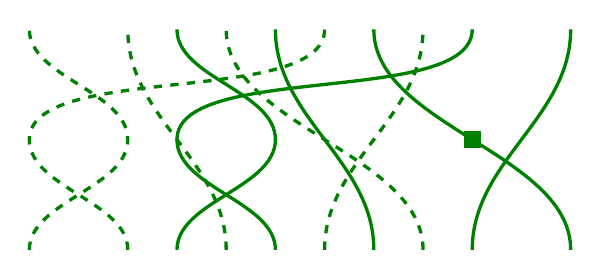
\begin{tikzpicture}[baseline,very thick,green!50!black, xscale=2.5,yscale=1.4]
 \draw (-.5,-1) to[out=90,in=-90] (-1,0) to[out=90,in=-90](.5,1);
 \draw[dashed] (-1.25,-1) to[out=90,in=-90] (-1.75,0) to[out=90,in=-90](-.25,1);
 \draw (.5,-1) to[out=90,in=-90] (1,1);
 \draw[dashed] (-.25,-1) to[out=90,in=-90] (.25,1);
 \draw (1,-1) to[out=90,in=-90] 
 node[midway,fill=green!50!black,inner sep=3pt]{} (0,1);
 \draw[dashed] (.25,-1) to[out=90,in=-90] (-.75,1);
 \draw (-1, -1) to[out=90,in=-90] (-.5,0) to[out=90,in=-90] (-1,1);
 \draw (0,-1) to[out=90,in=-90] (-.5,1);
 \draw[dashed] (-1.75, -1) to[out=90,in=-90] (-1.25,0) to[out=90,in=-90] (-1.75,1);
 \draw[dashed] (-.75,-1) to[out=90,in=-90] (-1.25,1);
\end{tikzpicture}\]

\begin{defi}\label{def:waha}
The rank $n$ \emph{type W affine Hecke algebra} (WAHA) $\waha_{\mathscr{B}}
(\pq)$ for some collection $\mathscr{B}$
of finite subsets $B_i\subset \R$ is the $\K\llbracket h\rrbracket $-span of all rank $n$ type W Hecke diagrams such that endpoints of the strands on the lines
$y=0$ and $y=1$ form a subset in $\mathscr{B}$, modulo the local relations:
\newseq
\begin{equation*}\subeqn\label{nilHecke-2}
 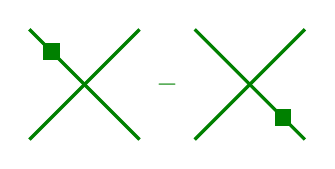
\begin{tikzpicture}[scale=.7,baseline,green!50!black]
 \draw[very thick](-3,0) +(-1,-1) -- +(1,1); \draw[very thick](-3,0) +(1,-1) --
 node[pos=.8,fill=green!50!black,inner sep=3pt]{} +(-1,1) ;
 % \draw[very thick] (0,0) +(0,-1) -- +(0,1) node[below, at
 % start]{$i$}; \fill (0,0) circle (5pt);
 \node at (-1.5,0){$-$}; \draw[very thick](0,0) +(-1,-1) -- +(1,1); \draw[very thick](0,0) +(1,-1) -- node[pos=.2,fill=green!50!black,inner sep=3pt]{}
 +(-1,1); 
 \end{tikzpicture}\hspace{4mm}=\hspace{4mm}
 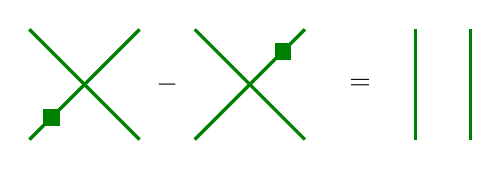
\begin{tikzpicture}[scale=.7,baseline]
 \draw[very thick,green!50!black](-3,0) +(-1,-1) -- node[pos=.2,fill=green!50!black,inner sep=3pt]{}+(1,1); \draw[very thick,green!50!black](-3,0) +(1,-1) -- +(-1,1); 
 % \draw[very thick] (0,0) +(0,-1) -- +(0,1) node[below, at
 % start]{$i$}; \fill (0,0) circle (5pt);
 \node at (-1.5,0){$-$}; \draw[very thick,green!50!black](0,0) +(-1,-1) --
 node[pos=.8,fill=green!50!black,inner sep=3pt]{} +(1,1); \draw[very thick,green!50!black](0,0) +(1,-1) -- +(-1,1)
 ; \node[black] at (2,0){$=$}; \draw[very
 thick,green!50!black](4,0) +(-1,-1) -- +(-1,1); \draw[very
 thick,green!50!black](4,0) +(0,-1) -- +(0,1); 
 \end{tikzpicture}
 \end{equation*}
 \begin{equation*}\subeqn\label{NilHecke3}
 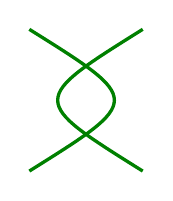
\begin{tikzpicture}[very thick,scale=.9,baseline,green!50!black]
 \draw(-2.8,0) +(0,-1) .. controls (-1.2,0) .. +(0,1)
 ; \draw (-1.2,0) +(0,-1) .. controls
 (-2.8,0) .. +(0,1) ; 
 \end{tikzpicture}\hspace{4mm}
= 0\qquad \qquad 
 
\begin{tikzpicture}[very thick,scale=.9,baseline,green!50!black]
 \draw (-3,0) +(1,-1) -- +(-1,1); \draw
 (-3,0) +(-1,-1) -- +(1,1) ; \draw
 (-3,0) +(0,-1) .. controls (-4,0) .. +(0,1); 
 \end{tikzpicture}\hspace{4mm}=\hspace{4mm}

\begin{tikzpicture}[very thick,scale=.9,baseline,green!50!black]
\draw (1,0) +(1,-1) -- +(-1,1)
 ; \draw (1,0) +(-1,-1) -- +(1,1)
 ; \draw (1,0) +(0,-1) .. controls
 (2,0) .. +(0,1); 
 \end{tikzpicture}\hspace{4mm}
 \end{equation*}
\[ \subeqn\label{green-ghost-bigon1}
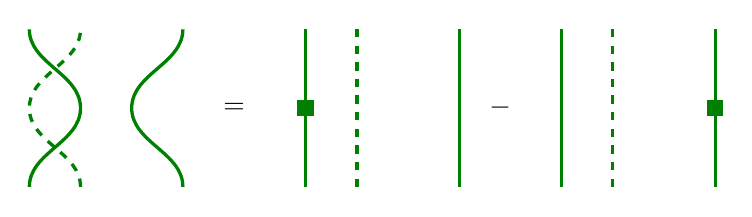
\begin{tikzpicture}[very thick,xscale=1.3,baseline=25pt,green!50!black]
 \draw (1,0) to[in=-90,out=90] (1.5,1) to[in=-90,out=90] (1,2)
;
 \draw[dashed] (1.5,0) to[in=-90,out=90] (1,1) to[in=-90,out=90] (1.5,2);
 \draw (2.5,0) to[in=-90,out=90] (2,1) to[in=-90,out=90] (2.5,2);
\node[black] at (3,1) {$=$};
 \draw (3.7,0) --node[midway,fill,inner sep=3pt]{} (3.7,2) 
 ;
 \draw[dashed] (4.2,0) to (4.2,2);
 \draw (5.2,0) -- (5.2,2);
\node[black] at (5.6,1) {$-\pq$};
 \draw (6.2,0) -- (6.2,2);
 \draw[dashed] (6.7,0)-- (6.7,2);
 \draw (7.7,0) -- node[midway,fill,inner sep=3pt]{} (7.7,2);
\end{tikzpicture}
\]
\[ \subeqn\label{green-ghost-bigon2}
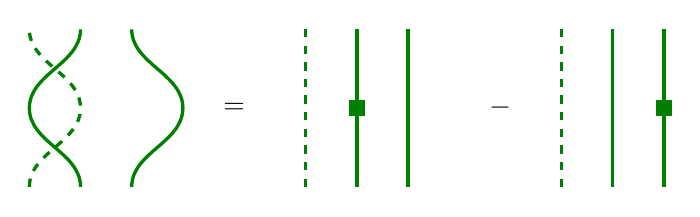
\begin{tikzpicture}[very thick,xscale=1.3,baseline=25pt,green!50!black]
 \draw[dashed] (1,0) to[in=-90,out=90] (1.5,1) to[in=-90,out=90] (1,2)
;
 \draw(1.5,0) to[in=-90,out=90] (1,1) to[in=-90,out=90] (1.5,2);
 \draw (2,0) to[in=-90,out=90] (2.5,1) to[in=-90,out=90] (2,2);
\node[black] at (3,1) {$=$};
 \draw[dashed] (3.7,0) --(3.7,2) 
 ;
 \draw (4.2,0) to node[midway,fill,inner sep=3pt]{} (4.2,2);
 \draw (4.7,0) -- (4.7,2);
\node[black] at (5.6,1) {$-\pq$};
 \draw[dashed] (6.2,0) -- (6.2,2);
 \draw (6.7,0)-- (6.7,2);
 \draw (7.2,0) -- node[midway,fill,inner sep=3pt]{} (7.2,2);
\end{tikzpicture}
\]
\begin{equation*}\label{eq:triple-point-1}\subeqn
 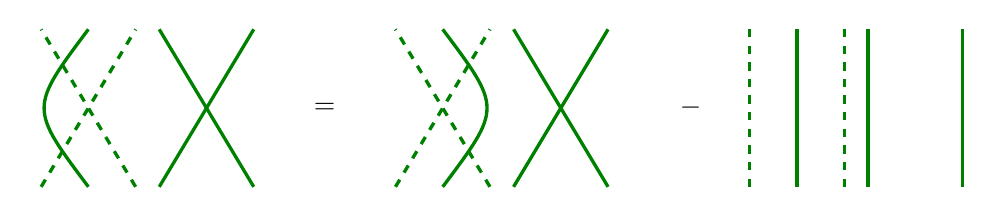
\begin{tikzpicture}[very thick,xscale=1.5,baseline,green!50!black]
 \draw[dashed] (-3,0) +(.4,-1) -- +(-.4,1);
 \draw[dashed] (-3,0) +(-.4,-1) -- +(.4,1); 
 \draw (-2,0) +(.4,-1) -- +(-.4,1); \draw
 (-2,0) +(-.4,-1) -- +(.4,1); 
 \draw (-3,0) +(0,-1) .. controls (-3.5,0) .. +(0,1);\node[black] at (-1,0) {=}; \draw[dashed] (0,0) +(.4,-1) -- +(-.4,1);
 \draw[dashed] (0,0) +(-.4,-1) -- +(.4,1); 
 \draw (1,0) +(.4,-1) -- +(-.4,1); \draw
 (1,0) +(-.4,-1) -- +(.4,1); 
 \draw (0,0) +(0,-1) .. controls (.5,0) .. +(0,1);
\node[black] at (2.1,0) {$-\pq$};
 \draw (4,0)
 +(.4,-1) -- +(.4,1); \draw (4,0)
 +(-.4,-1) -- +(-.4,1); 
 \draw[dashed] (3,0)
 +(.4,-1) -- +(.4,1); \draw[dashed] (3,0)
 +(-.4,-1) -- +(-.4,1); 
\draw (3,0)
 +(0,-1) -- +(0,1);
 \end{tikzpicture}
 \end{equation*}
\begin{equation*}\label{eq:triple-point-2}\subeqn
 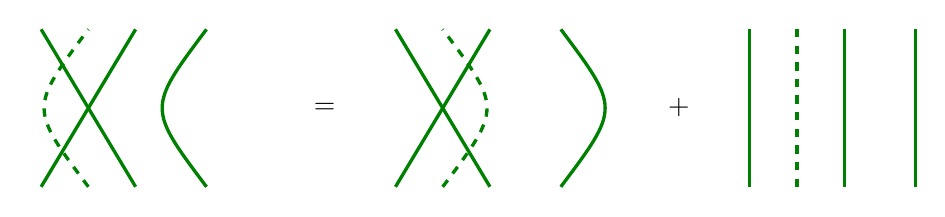
\begin{tikzpicture}[very thick,xscale=1.5,baseline,green!50!black]
 \draw (-3,0) +(.4,-1) -- +(-.4,1);
 \draw (-3,0) +(-.4,-1) -- +(.4,1); 
\draw (-2,0) +(0,-1) .. controls (-2.5,0) .. +(0,1);
 \draw[dashed] (-3,0) +(0,-1) .. controls (-3.5,0) .. +(0,1);\node[black] at (-1,0) {$=$}; \draw (0,0) +(.4,-1) -- +(-.4,1);
 \draw (0,0) +(-.4,-1) -- +(.4,1); 
 \draw[dashed] (0,0) +(0,-1) .. controls (.5,0) .. +(0,1);
 \draw (1,0) +(0,-1) .. controls (1.5,0) .. +(0,1);
\node[black] at (2,0)
 {$+$}; 
 \draw (3,0)
 +(.4,-1) -- +(.4,1); \draw (3,0)
 +(-.4,-1) -- +(-.4,1); 
 \draw[dashed] (3,0)
 +(0,-1) -- +(0,1); \draw (4,0)
 +(0,-1) -- +(0,1); 
 \end{tikzpicture}
 \end{equation*}

\end{defi}
\begin{rema}
 As in the type O case, this algebra also has a degenerate analogue,
 where we replace
 (\ref{green-ghost-bigon1}--\ref{eq:triple-point-1}) with the
 equations 
\[ \subeqn\label{deg-green-ghost-bigon1}
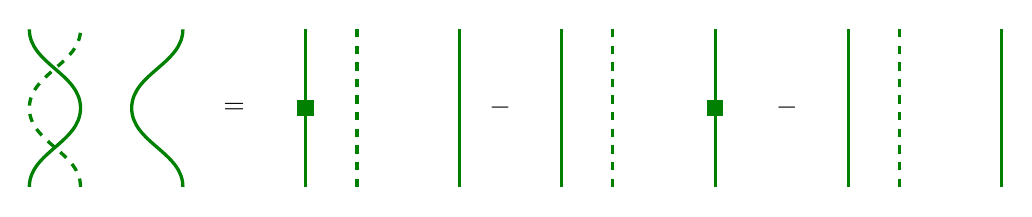
\begin{tikzpicture}[very thick,xscale=1.3,baseline=25pt,green!50!black]
 \draw (1,0) to[in=-90,out=90] (1.5,1) to[in=-90,out=90] (1,2)
;
 \draw[dashed] (1.5,0) to[in=-90,out=90] (1,1) to[in=-90,out=90] (1.5,2);
 \draw (2.5,0) to[in=-90,out=90] (2,1) to[in=-90,out=90] (2.5,2);
\node[black] at (3,1) {$=$};
 \draw (3.7,0) --node[midway,fill,inner sep=3pt]{} (3.7,2) 
 ;
 \draw[dashed] (4.2,0) to (4.2,2);
 \draw (5.2,0) -- (5.2,2);
\node[black] at (5.6,1) {$-$};
 \draw (6.2,0) -- (6.2,2);
 \draw[dashed] (6.7,0)-- (6.7,2);
 \draw (7.7,0) -- node[midway,fill,inner sep=3pt]{} (7.7,2);
\node[black] at (8.4,1) {$-$};
 \draw (9,0) -- (9,2);
 \draw[dashed] (9.5,0)-- (9.5,2);
 \draw (10.5,0) -- (10.5,2);
\end{tikzpicture}
\]
\[ \subeqn\label{deg-green-ghost-bigon2}
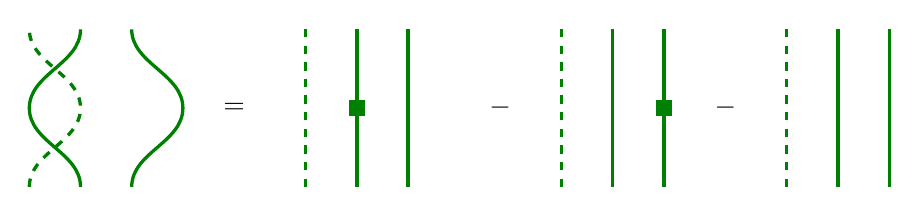
\begin{tikzpicture}[very thick,xscale=1.3,baseline=25pt,green!50!black]
 \draw[dashed] (1,0) to[in=-90,out=90] (1.5,1) to[in=-90,out=90] (1,2)
;
 \draw(1.5,0) to[in=-90,out=90] (1,1) to[in=-90,out=90] (1.5,2);
 \draw (2,0) to[in=-90,out=90] (2.5,1) to[in=-90,out=90] (2,2);
\node[black] at (3,1) {$=$};
 \draw[dashed] (3.7,0) --(3.7,2) 
 ;
 \draw (4.2,0) to node[midway,fill,inner sep=3pt]{} (4.2,2);
 \draw (4.7,0) -- (4.7,2);
\node[black] at (5.6,1) {$-$};
 \draw[dashed] (6.2,0) -- (6.2,2);
 \draw (6.7,0)-- (6.7,2);
 \draw (7.2,0) -- node[midway,fill,inner sep=3pt]{} (7.2,2);
\node[black] at (7.8,1) {$-$};
 \draw[dashed] (8.4,0) -- (8.4,2);
 \draw (8.9,0)-- (8.9,2);
 \draw (9.4,0) -- (9.4,2);
\end{tikzpicture}
\]
\begin{equation*}\label{eq:deg-triple-point-1}\subeqn
 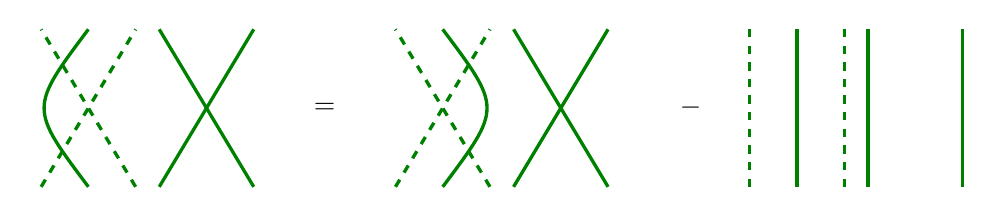
\begin{tikzpicture}[very thick,xscale=1.5,baseline,green!50!black]
 \draw[dashed] (-3,0) +(.4,-1) -- +(-.4,1);
 \draw[dashed] (-3,0) +(-.4,-1) -- +(.4,1); 
 \draw (-2,0) +(.4,-1) -- +(-.4,1); \draw
 (-2,0) +(-.4,-1) -- +(.4,1); 
 \draw (-3,0) +(0,-1) .. controls (-3.5,0) .. +(0,1);\node[black] at (-1,0) {=}; \draw[dashed] (0,0) +(.4,-1) -- +(-.4,1);
 \draw[dashed] (0,0) +(-.4,-1) -- +(.4,1); 
 \draw (1,0) +(.4,-1) -- +(-.4,1); \draw
 (1,0) +(-.4,-1) -- +(.4,1); 
 \draw (0,0) +(0,-1) .. controls (.5,0) .. +(0,1);
\node[black] at (2.1,0) {$-$};
 \draw (4,0)
 +(.4,-1) -- +(.4,1); \draw (4,0)
 +(-.4,-1) -- +(-.4,1); 
 \draw[dashed] (3,0)
 +(.4,-1) -- +(.4,1); \draw[dashed] (3,0)
 +(-.4,-1) -- +(-.4,1); 
\draw (3,0)
 +(0,-1) -- +(0,1);
 \end{tikzpicture}
 \end{equation*}
\end{rema}

By convention, we'll let $e_{B}$ be the diagram with vertical lines at
$x=b$ for $b\in B$, and use $X_i$ to represent the square on the $i$th
strand from left.
\begin{prop}\label{W-poly}
 The WAHA $\waha_{\mathscr{B}}(\pq)$ for a set $\mathscr{B}$ has a polynomial representation
 \[P_{\mathscr{B}} := \oplus_{B\in \mathscr{B}}\K\llbracket h\rrbracket [Y_1^{\pm 1},\dots,
 Y_{|B|}^{\pm 1}]\]
defined by the rule that 
\begin{itemize}
\item Each crossing of the $r$ and $r+1$st strands acts by the Demazure operator \[\partial_r(F)=
 \frac{F^{s_r}-F}{Y_{r+1}-Y_{r}}.\]
\item 
A crossing between the $r$th strand and a ghost of $s$th strand acts
by
\begin{itemize}
\item the identity if $\ck <0$ and the
 strand is NE/SW or $\ck >0$ and the strand is NW/SE,
\item the multiplication operator of $Y_r-qY_s$ if $\ck <0$ and
 the strand is NW/SE or $\ck >0$ and the strand is NE/SW
\end{itemize}
\item A square on the $r$th strand acts by the multiplication operator
 $Y_r$. 
\end{itemize}
\end{prop}
\begin{proof}
The equations (\ref{nilHecke-2}--\ref{NilHecke3}) are the usual
relations satisfied by multiplication and Demazure operators. The 
equations (\ref{green-ghost-bigon1}--\ref{green-ghost-bigon2}) are clear from
the definition of the operators for ghost/strand crossings. Finally,
the relations (\ref{eq:triple-point-1}--\ref{eq:triple-point-2}) are
calculation with Demazure operators similar to that which is standard
for triple points in various KLR calculi.
For example, assuming $\ck<0$ for~\eqref{eq:triple-point-1}, the
LHS is \[\partial_s\circ (Y_r-qY_s)=(Y_r-qY_{s+1})\circ\partial_s-q\]
using the usual twisted Leibnitz rule for Demazure operators; this is
the RHS, so we are done. On the other hand,
\eqref{eq:triple-point-2}~follows in a similar way from the equation
\[(Y_r-qY_s)\circ\partial_r = \partial_r \circ (Y_{r+1}-qY_s)+1.\] This
completes the proof.
\end{proof}

\begin{prop}\label{prop:waha-basis}
 The rank $n$ type W Hecke algebra $\waha_{\mathscr{B}}(\pq)$ has a basis over $\K\llbracket h\rrbracket $ given by the products
 $e_{B}D_wX_1^{a_1}\cdots X_n^{a_n}e_{B'}$ for $w\in S_n$ and $(a_1,\dots,
 a_n)\in \Z^n$; here $D_w$ is a arbitrarily chosen diagram which
 induces the permutation $w$ on the endpoints at $y=0$ when they are
 associated to the endpoint at the top of same strand, and no pair of
 strands or ghosts cross twice.

 The action of $\waha_{\mathscr{B}}(\pq)$ on its polynomial
 representation is faithful.
\end{prop}
\begin{proof}
 This proof follows many similar ones in KLR theory. These elements
 are linearly independent because the elements $D_w$ span the action
 of $\K[S_n]$ after extending scalars to the fraction field of
 rational functions, since $D_w=f_w w+\sum_{v<w} f_v v$ for some
 rational functions $f_v$ with $f_w\neq 0$. Thus our proposed basis
 is linearly independent over $\K$ in this scalar extension, so must
 have been linearly independent before.

 Note that this shows that the action of these elements on the
 polynomial representation is linearly independent. Thus, if we show
 that they span, it will show that the representation is faithful. 

 Now we need only show that they span. Using relation
~\eqref{nilHecke-2}, we can assume that all squares are at the bottom
 of the diagram. 

Furthermore, any two choices of the diagram $D_w$ differ via a series
of isotopies and triple points, so relations
(\ref{NilHecke3},\ref{eq:triple-point-1},\ref{eq:triple-point-2}) show
that these diagrams differ by diagrams with fewer crossings between
strands and ghosts. Thus, we
need only show that any diagram with a bigon can be written as a sum
of diagrams with fewer crossings. 

Now, assume we have such a bigon. We should assume that it has no
smaller bigons inside it. In this case, we can shrink the bigon,
using the relations
(\ref{NilHecke3},\ref{eq:triple-point-1},\ref{eq:triple-point-2})
whenever we need to move a strand through the top and bottom of the
bigon or a crossing out through its side. Thus, we can ultimately
assume that the bigon is empty, and apply the relations (\ref{NilHecke3}--\ref{green-ghost-bigon2}).
\end{proof}

We now have the results we need to apply the results of Section
\ref{sec:polyn-style-repr}, in the case of
\begin{equation}
\mathbb{K}=\K\llbracket h\rrbracket \quad A=\waha_{\mathscr{B}}(\pq)\quad
 B=\K\llbracket h\rrbracket [X^{\pm}]\quad I=Bh+B \prod_{u\in \gls{U}}(X-u)\quad P=\mathcal{P}_{\mathscr{B}}.\label{eq:wHecke-PR}
\end{equation}
The requisite freeness and the faithfulness of the polynomial
representation follow from Proposition
\ref{prop:waha-basis}, so this defines a polynomial style
representation. Thus, we have an induced completion
$\gls{hwaha}_{\mathscr{B}}$ with faithful completed polynomial
representation by Lemma~\ref{lem:faithful-completion}.


\subsubsection{Comparison with Hecke and Schur algebras}
\label{sec:comp-with-hecke}

Choose 
$$
\wellsep =  \{B_s  =  \{s,2s,3s,\dots, ns\}\}
$$
 for $s$ some real
number with $s\gg |g|$. For every type O diagram on $n$ strands,
we can choose an isotopy representative such that the endpoints of the
diagram are precisely $B_s$ at both $y=0$ and $y=1$. Furthermore, we
can choose this representative so that if we think of it as a type W
diagram and add ghosts, no strand is between a crossing
of strands and the corresponding ghost crossing. Obviously we can do
this for individual crossings, and any diagram can be factored into
these.
\begin{theorem}\label{wdHecke}
 This embedding induces an isomorphism between the WAHA $\waha_{\wellsep}(\pq)$ and
 the honest affine Hecke algebra
 $\gls{mH}(\pq)$:
 \begin{itemize}
 \item If $\ck <0$, this isomorphism sends a single crossing to
 $T_i+1$. That is, the diagrams satisfy the local relations
 (\ref{Hecke-1}--\ref{Hecke-triple}).
\item If $\ck>0$, this
 isomorphism sends a single crossing to $T_i-q$. That is, the diagrams satisfy the local relations
 (\ref{qHecke-1}--\ref{qHecke-triple}).
 \end{itemize}
The polynomial representation defined above
 is intertwined by this map with the polynomial representation of
 $\gls{mH}(\pq)$ if $\ck <0$ and the signed polynomial representation if $\ck>0$. 
\end{theorem}
This theorem shows that if we view type O diagrams as type W diagrams
where $|\ck|$ is sufficiently small that we cannot distinguish
between a strand and its ghost\footnote{Perhaps this will be easier if
 you take off your glasses.}, then the local relations
(\ref{Hecke-1}--\ref{Hecke-triple}) will be consequences of (\ref{nilHecke-2}--\ref{eq:triple-point-2}).
\begin{proof}
We'll consider the case where $\ck <0$. We have that $T_i+1$ is sent to the diagram 
\begin{equation*}
 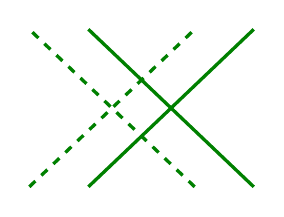
\begin{tikzpicture}[very thick,xscale=1.5,baseline,green!50!black]
 \draw (-2.5,0) +(.7,-1) -- +(-.7,1);
 \draw (-2.5,0) +(-.7,-1) -- +(.7,1); 
 \draw[dashed] (-3,0) +(.7,-1) -- +(-.7,1);
 \draw [dashed] (-3,0) +(-.7,-1) -- +(.7,1); 
 \end{tikzpicture}
 \end{equation*}
which sent by the polynomial representation of the type W affine Hecke algebra
 representation to $(Y_r-\pq Y_{r+1}) \circ \partial_r$. That is, we
 have $T_iF=-F^{s_r}+(1-\pq)Y_{r+1}\partial_r$. Since
 $\waha_{\mathscr{B}}(\pq)$ acts faithfully on its polynomial representation,
 this shows that we have a map of the Hecke algebra to the WAHA; the
 faithfulness of $\cP^-$ implies that this map is injective. 
 Since the diagram $D_w$ and the polynomials in the squares are in
 the image of this map, the map is surjective. 

The case $\ck>0$ follows similarly.
\end{proof}
Thus, the WAHA for any set containing $\wellsep$ is a ``larger'' algebra than the affine Hecke
algebra. The category of representations of affine Hecke algebras are
a quotient category of its representations via the functor $M\mapsto e_{\wellsep}M$, though in some cases, this
quotient will be an equivalence. 

For any composition $\Bk=(k_1,\dots, k_n)$ of $m$, we have an associated
quasi-idempotent $\epsilon_{\Bk}=\sum_{w\in S_{\Bk}}T_w$ symmetrizing for the associated Young
subgroup. If $\Bk=(1,\dots, 1)$, then $\epsilon_{\Bk}=1$.

\begin{defi}\label{def:cS}
 The \emph{affine $q$-Schur algebra} $\cS(\pq,n,m)$, as defined in
~\cite[Def.~2.1.4]{GreenSchur}, is the algebra defined
 by
 \[\cS(\pq,n,m):=
 \End_{\gls{mH}(\pq)}\left(\bigoplus_{|\Bk|=m}\epsilon_{\Bk}\gls{mH}(\pq)
 \right)%=\bigoplus_{|\Bk|=|\Bk'|=n}\epsilon_{\Bk}\gls{mH}\cap \gls{mH}\epsilon_{\Bk'},
 \] where the sum is over $n$-part compositions of $m$.
\end{defi}
Following~\cite{GreenSchur}, we let $E(n,m)$ denote the $\cS(\pq,n,m)$-$\gls{mH}(\pq)$ bimodule $\bigoplus_{|\Bk|=m}\epsilon_{\Bk}\gls{mH}(\pq)$.


By a result of Jimbo~\cite{Jimbo}, the affine Hecke algebra acts naturally on $M\otimes V^{\otimes n}$ for any finite
dimensional $U_{\pq}(\mathfrak{gl}_n)$-module $M$ and $V$ the defining
representation using universal R-matrices and Casimir operators; analogously, the
algebra $\cS(\pq,n,m)$ naturally acts on
\[\bigoplus _{|\Bk|=m}M\otimes \Sym^{ k_1}V\otimes \cdots\otimes
\Sym^{k_n}V\cong E(n,m)\otimes_{\gls{mH}(\pq)}M\otimes V^{\otimes n}.\]
Furthermore, the algebra $\cS(\pq,n,m)$ has a natural 
polynomial representation given by
\[\cP_{\cS}:=\bigoplus_{|\Bk|=m}
 \cP^{S_{\Bk}}\cong E(n,m)\otimes_{\gls{mH}(\pq)}\cP^-.\]
There is a more detailed exposition of this representation in~\cite[\S~4]{MiSt}.
\begin{lemma}
 This representation is faithful.
\end{lemma}
\begin{proof}
 The algebra $\cS(\pq,n,m)$ have a basis $\phi^d_{\Bk,\Bk'}$ defined in
~\cite[Def.~2.2.3]{GreenSchur}. This element is defined as a linear
 combination of left multiplications of elements of $\gls{mH}(\pq)$,
 restricted to $\epsilon_{\Bk}\gls{mH}(\pq)$. Thus, any non-trivial linear
 combination of these elements has the same property.
 By the faithfulness of
 $\cP^-$, this implies that no non-trivial linear combination of
 $\phi^d_{\Bk,\Bk'}$ acts trivially. That is, the action is
 faithful. 
\end{proof}


If we replace $\epsilon_{\Bk}$ by the anti-symmetrizing quasi-idempotent
$\epsilon_{\Bk}^-\Mk =\Mk \sum_{w\in S_{\Bk}} (\mk -\mk q)^{\ell(w)}T_w$, then we obtain the signed
$q$-Schur algebra $\cS_h^-(n,m)$, which instead acts on \[\bigoplus
_{|\Bk|=m}M\otimes \iwedge{ k_1}V\otimes \cdots\otimes
\iwedge{k_n}V.\]

The affine $q$-Schur algebra has a diagrammatic realization much like the
affine Hecke algebra. For each composition $\mu=(\mu_1,\dots, \mu_n)$
of $m$, we let $C_\mu=\{i\epsilon+js\mid 0\leq i< \mu_j\}$ for some
fixed $0< \epsilon \ll g \ll s$, and let $\gls{Cset}$ be the
collection of these sets. That is, we have groups of dots
corresponding to the parts of the composition, with sizes given by
$\mu_i$. 

In the type W affine Hecke algebra
$\waha_{\gls{Cset}}(\pq)$, we have an idempotent $e'_\mu$ which on each
group in $[js,js+\mu_j\epsilon]$ traces out the primitive idempotent
in the nilHecke algebra which acts as $\partial_{w_0} y^{\mu_j-1}_1\cdots
y_{\mu_j-1}$ in the polynomial representation. For example, for
$\mu=(1,3,2)$, this idempotent is given by:
\[

\begin{tikzpicture}[very thick,xscale=1.5,baseline,green!50!black]
 \draw (0,-1) -- (0,1);
 \draw (4,-1) to[out=90,in=-90] node[pos=.2,fill=green!50!black,inner
 sep=3pt]{} (4.4, 1);
 \draw (4.4,-1) to[out=90,in=-90] (4, 1);
 \draw (2,-1) to[out=90,in=-90] node[pos=.35,fill=green!50!black,inner
 sep=3pt]{}node[pos=.175,fill=green!50!black,inner
 sep=3pt]{} (2.8, 1);
 \draw (2.8,-1) to[out=90,in=-90] (2, 1);
 \draw (2.4,-1) .. controls (2.9,0) .. node[pos=.1,fill=green!50!black,inner
 sep=3pt]{} (2.4, 1);
\end{tikzpicture}
\]
 Let
$\gls{eprime}=\sum_\mu e'_\mu$ be the sum of these idempotents over $m$-part
compositions of $n$.

\begin{theorem}\label{waha-Schur}
If $\ck<0$, we have an isomorphism of algebras $\gls{eprime} \waha_{\gls{Cset}}(\pq) \gls{eprime}\cong \cS(\pq,n,m)$
 which induces an isomorphism of representations $\gls{eprime}
 P_{\gls{Cset}}\cong \cP_{\cS(\pq,n,m)}$. Similarly, if $\ck>0$, we have an
 isomorphism of algebras $\gls{eprime} \waha_{\gls{Cset}}(\pq) \gls{eprime}\cong \cS_h^-(n,m)$.
\end{theorem}

 Setting $h=0$, we obtain an isomorphism between the WAHA $\gls{eprime} \waha_{\gls{Cset}}(\pq) \gls{eprime}$ (at $h=0$)
 with the usual affine Schur algebra for any field $\K$ and any
 $q\notin\{0,1\}$. Since this isomorphism requires passing through a
 Morita equivalence, it is quite difficult to make it explicit. A
 closely related isomorphism is shown in much greater detail by
 Miemietz and Stroppel in~\cite{MiSt}, relating the affine Schur
 algebra and the quiver Schur algebra from~\cite{SWschur}; presumably
 these results can ultimately be matched by tracing through the
 Morita equivalence of~\cite[Th.~3.8]{WebwKLR}, but we will not trace
 through the details of doing so. 

\begin{proof}
First, consider the case $\ck<0$. Consider the idempotent $e_{B_s}$ in $\gls{eprime} \waha_{\gls{Cset}}(\pq) \gls{eprime}$. This
satisfies $e_{B_s}\waha_{\gls{Cset}}(\pq)e_{B_s}\cong \gls{mH}(\pq)$ by Theorem~\ref{wdHecke}.

Thus, $\gls{eprime}e_{C_\mu}\waha_{\gls{Cset}}(\pq)e_{B_s}$ is naturally a right module
over $\gls{mH}(\pq)$. We wish to show that it is isomorphic to $\epsilon_\mu
\gls{mH}(\pq)$. Consider the diagram $e_{C_\mu}D_1e_{B_s}$. Acting on the
right by $T_i+1$ with $(i,i+1)\in S_{\mu_1}\times \cdots \times S_{\mu_p}$ gives $e_{C_\mu}D_ee_{B_s}(T_i+1)=(q+1)
e_{C_\mu}D_1e_{B_s}$, since
\begin{equation*}
 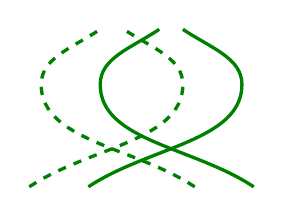
\begin{tikzpicture}[very thick,xscale=1.5,baseline,green!50!black]
 \draw (.7,-1) to [out=135,in=-90] (-.6,.3) to
 [out=90,in=-135] (-.1,1) ;
 \draw (-.7,-1)to [out=45,in=-90] (.6,.3) to
 [out=90,in=-45] (.1,1); 
 \draw[dashed] (.2,-1) to [out=135,in=-90] (-1.1,.3) to
 [out=90,in=-135] (-.6,1) ;
 \draw [dashed] (-1.2,-1) to [out=45,in=-90] (.1,.3) to
 [out=90,in=-45] (-.4,1) ;
 \end{tikzpicture}\hspace{4mm}=\hspace{4mm}
 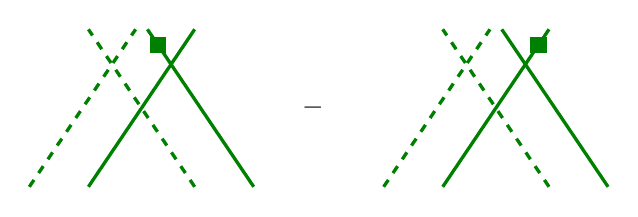
\begin{tikzpicture}[xscale=1.5,baseline,green!50!black]
 \draw[very thick](-3,0) +(-.7,-1) -- +(.2,1); \draw[very thick](-3,0) +(.7,-1) -- node[pos=.9,fill=green!50!black,inner
 sep=3pt]{}+(-.2,1)
 ; \draw[very thick,dashed](-3.5,0) +(-.7,-1) -- +(.2,1);
 \draw[very thick,dashed](-3.5,0)+(.7,-1) -- +(-.2,1) ;
 % \draw[very thick] (0,0) +(0,-1) -- +(0,1) node[below, at
 % start]{$i$}; \fill (0,0) circle (5pt);
 \node[black] at (-1.8,0){$-\pq$}; \draw[very thick](0,0) +(-.7,-1) -- node[pos=.9,fill=green!50!black,inner sep=3pt]{}+(.2,1); \draw[very thick](0,0) +(.7,-1) -- 
 +(-.2,1); 
\draw[very thick,dashed](-.5,0) +(-.7,-1) -- +(.2,1);
\draw[very thick,dashed] (-.5,0) +(.7,-1) -- +(-.2,1);
 \end{tikzpicture}
 \end{equation*}
Applying~\eqref{nilHecke-2}, the RHS is equal to $1+q$ times the
identity, plus diagrams with a crossing at top, which are killed by $\gls{eprime}$. This shows that
$\gls{eprime}e_{C_\mu}D_1e_{B_s}$ is invariant. Thus, we have a map of
$\epsilon_\mu \gls{mH}(\pq)\to \gls{eprime}e_{C_\mu}\waha_{\gls{Cset}}(\pq)e_{B_s}$ sending
$\epsilon_\mu \mapsto \gls{eprime}e_{C_\mu}D_ee_{B_s}$. This map must be
surjective, since every $ \gls{eprime}e_{C_\mu}D_we_{B_s}$ is in its image, and
comparing ranks over the fraction field $K=\K(X_1,\dots, X_n)$, we see that it
must be injective as well. Thus, the action of $\gls{eprime} \waha_{\gls{Cset}}(\pq) \gls{eprime}$
on $\gls{eprime} \waha_{\gls{Cset}}(\pq) e_{B_s}$ defines a map $\gls{eprime} \waha_{\gls{Cset}}(\pq) \gls{eprime}\to
\cS_h$. 

Assume $a\neq 0$ is in the kernel of this map 
$\gls{eprime} \waha_{\gls{Cset}}(\pq) \gls{eprime}$; that is, $a$ acts trivially on $\gls{eprime}
\waha_{\gls{Cset}}(\pq) e_{B_s}$. Note that
$\waha_{\gls{Cset}}(\pq)$ acts faithfully on the rational representation
$P^K_{\gls{Cset}}=P_{\gls{Cset}}\otimes_{\K[X_1^{\pm 1},\dots,X_n^{\pm 1}]}K$, and the element $D_1$ induces an isomorphism $
e_{C_{\mu} }P_{\gls{Cset}}^K\otimes F\to e_{B_s }P_{\gls{Cset}}^K\otimes
F$. Thus, we must have that $aD_1$ then acts non-trivially in $ e_{B_s }P_{\gls{Cset}}$, and so $aD_1e_{B_s }\neq 0$, contradicting our assumption that
$a$ is in the kernel.
Thus, we can only have $a=0$, and the map to the Schur algebra is injective.

On the other hand, note that the element $\gls{eprime}e_{C_\mu}D_we_{C_{\mu'}}e$
for $w$ any shortest double coset representative is sent to the element
$\phi_w=\sum_{w'\in S_{\mu}w S_{\mu'}}T_{w'}$ plus elements in
$\K\llbracket h\rrbracket [X^{\pm 1}_1,\dots, X^{\pm 1}_n]\phi_v$ for $v$ shorter in Bruhat
order. Since $\phi_w X^{a_1}_1,\dots, X^{a_n}_n$ give a basis of
$\cS_h$ by~\cite[2.2.2]{GreenSchur}, the fact that these are in the image shows that this map is
surjective.

When $\ck >0$, the argument is quite similar, but with $T_i-q$
replacing $T_i+1$ and using the $\ck>0$ version of Theorem~\ref{wdHecke}.
\end{proof}
We'll prove in Corollary~\ref{affine-schur-morita} that the idempotent
$\gls{eprime}$ induces a Morita equivalence between $\waha_{\gls{Cset}}$ and $\gls{cS}_h(n,m)$.
Thus, from the perspective of the Hecke side, introducing the type W
relations is an alternate way of understanding the affine Schur
algebra.

\subsection{Weighted KLR algebras}
\label{sec:weight-klr-algebr}


On the other hand, the author has incorporated similar ideas
into the theory of KLR algebras, by introducing \emph{weighted KLR
 algebras}~\cite{WebwKLR}.
\begin{defi}\label{def:wKLR}
 Let $\gls{W}(\pq)$ be the rank $n$ weighted KLR algebra attached to the graph $\gls{U}$; that
 is, $\gls{W}(\pq)$ is the quotient of $\K[h]$-span of weighted KLR
 diagrams with $n$ strands
 (as defined in~\cite[Def.~2.3]{WebwKLR}) by the local relations
 (note that these relations are drawn with $\ck<0$): \newseq
 \begin{equation*}\subeqn\label{dots-1}%%%a
 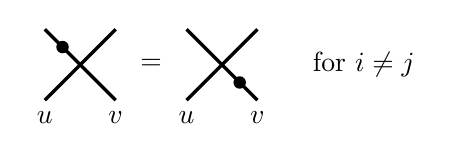
\begin{tikzpicture}[scale=.45,baseline]
 \draw[very thick](-4,0) +(-1,-1) -- +(1,1) node[below,at start]
 {$u$}; \draw[very thick](-4,0) +(1,-1) -- +(-1,1) node[below,at
 start] {$v$}; \fill (-4.5,.5) circle (5pt);
 % \draw[very thick] (0,0) +(0,-1) -- +(0,1) node[below, at
 % start]{$u$}; \fill (0,0) circle (5pt);
 \node at (-2,0){=}; \draw[very thick](0,0) +(-1,-1) -- +(1,1)
 node[below,at start] {$u$}; \draw[very thick](0,0) +(1,-1) --
 +(-1,1) node[below,at start] {$v$}; \fill (.5,-.5) circle (5pt);
 \node at (4,0){for $i\neq j$};
 \end{tikzpicture}\end{equation*}
 \begin{equation*}\label{dots-2}\subeqn%%%%b
 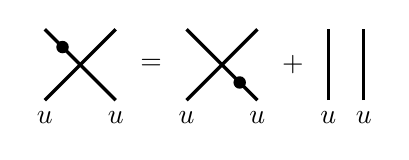
\begin{tikzpicture}[scale=.45,baseline]
 \draw[very thick](-4,0) +(-1,-1) -- +(1,1) node[below,at start]
 {$u$}; \draw[very thick](-4,0) +(1,-1) -- +(-1,1) node[below,at
 start] {$u$}; \fill (-4.5,.5) circle (5pt);
 % \draw[very thick] (0,0) +(0,-1) -- +(0,1) node[below, at
 % start]{$u$}; \fill (0,0) circle (5pt);
 \node at (-2,0){=}; \draw[very thick](0,0) +(-1,-1) -- +(1,1)
 node[below,at start] {$u$}; \draw[very thick](0,0) +(1,-1) --
 +(-1,1) node[below,at start] {$u$}; \fill (.5,-.5) circle (5pt);
 \node at (2,0){+}; \draw[very thick](4,0) +(-1,-1) -- +(-1,1)
 node[below,at start] {$u$}; \draw[very thick](4,0) +(0,-1) --
 +(0,1) node[below,at start] {$u$};
 \end{tikzpicture}\qquad
 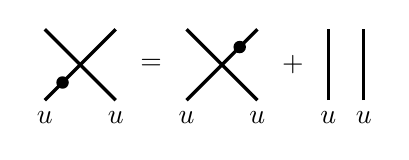
\begin{tikzpicture}[scale=.45,baseline]
 \draw[very thick](-4,0) +(-1,-1) -- +(1,1) node[below,at start]
 {$u$}; \draw[very thick](-4,0) +(1,-1) -- +(-1,1) node[below,at
 start] {$u$}; \fill (-4.5,-.5) circle (5pt);
 % \draw[very thick] (0,0) +(0,-1) -- +(0,1) node[below, at
 % start]{$u$}; \fill (0,0) circle (5pt);
 \node at (-2,0){=}; \draw[very thick](0,0) +(-1,-1) -- +(1,1)
 node[below,at start] {$u$}; \draw[very thick](0,0) +(1,-1) --
 +(-1,1) node[below,at start] {$u$}; \fill (.5,.5) circle (5pt);
 \node at (2,0){+}; \draw[very thick](4,0) +(-1,-1) -- +(-1,1)
 node[below,at start] {$u$}; \draw[very thick](4,0) +(0,-1) --
 +(0,1) node[below,at start] {$u$};
 \end{tikzpicture}
 \end{equation*}
 \begin{equation*}\label{strand-bigon}\subeqn %%%%c
 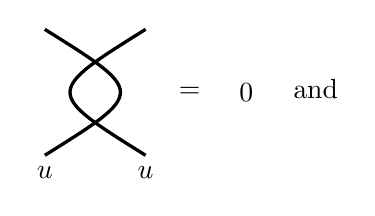
\begin{tikzpicture}[very thick,scale=.8,baseline]
 \draw (-2.8,0) +(0,-1) .. controls (-1.2,0) .. +(0,1)
 node[below,at start]{$u$}; \draw (-1.2,0) +(0,-1) .. controls
 (-2.8,0) .. +(0,1) node[below,at start]{$u$}; \node at (-.5,0)
 {=}; \node at (0.4,0) {$0$}; \node at (1.5,.05) {and};
 \end{tikzpicture}
 \hspace{.4cm}
 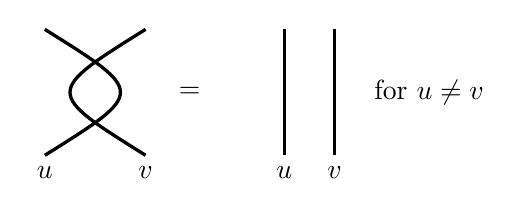
\begin{tikzpicture}[very thick,scale=.8 ,baseline]

 \draw (-2.8,0) +(0,-1) .. controls (-1.2,0) .. +(0,1)
 node[below,at start]{$u$}; \draw (-1.2,0) +(0,-1) .. controls
 (-2.8,0) .. +(0,1) node[below,at start]{$v$}; \node at (-.5,0)
 {=};


 \draw (1.8,0) +(0,-1) -- +(0,1) node[below,at start]{$v$}; \draw
 (1,0) +(0,-1) -- +(0,1) node[below,at start]{$u$};\node at (3.3,0){for $u\neq v$};
 \end{tikzpicture}
 \end{equation*} 
\refstepcounter{subeqn} 
 \begin{multline*}\label{ghost-bigon1}\subeqn%%%%d
 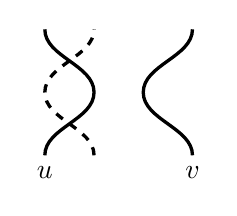
\begin{tikzpicture}[very thick,xscale=1.25 ,yscale=.8,baseline]
 \draw (1,-1) to[in=-90,out=90] node[below, at start]{$u$}
 (1.5,0) to[in=-90,out=90] (1,1) ; \draw[dashed] (1.5,-1)
 to[in=-90,out=90] (1,0) to[in=-90,out=90] (1.5,1); \draw
 (2.5,-1) to[in=-90,out=90] node[below, at start]{$v$} (2,0)
 to[in=-90,out=90] (2.5,1); 
 \end{tikzpicture}
 \\
 \begin{tikzpicture}[very thick,xscale=1.25 ,yscale=.8,baseline]
\node at (3,0) {=}; 
 \end{tikzpicture}
 \begin{cases}
 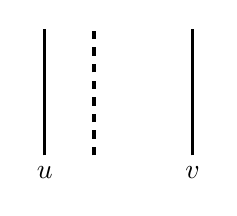
\begin{tikzpicture}[very thick,xscale=1.25 ,yscale=.8,baseline]
\draw (3.7,-1) --
 (3.7,1) node[below, at start]{$u$} ; \draw[dashed] (4.2,-1) to
 (4.2,1); \draw (5.2,-1) -- (5.2,1) node[below, at start]{$v$};
 \end{tikzpicture} & \text{for $u\neq qv$}\\
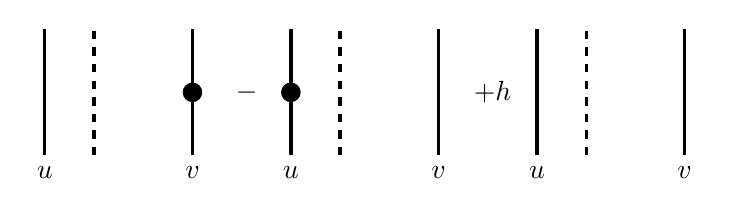
\begin{tikzpicture}[very thick,xscale=1.25,yscale=.8,baseline]
 \draw (3.7,-1) --
 (3.7,1) node[below, at start]{$u$} ; \draw[dashed] (4.2,-1) to
 (4.2,1); \draw (5.2,-1) -- (5.2,1) node[below, at start]{$v$}
 node[midway,fill,inner sep=2.5pt,circle]{}; \node at (5.75,0)
 {$-$};
 \draw (6.2,-1) -- (6.2,1) node[below, at start]{$u$}
 node[midway,fill,inner sep=2.5pt,circle]{}; \draw[dashed]
 (6.7,-1)-- (6.7,1); \draw (7.7,-1) -- (7.7,1) node[below, at
 start]{$v$};
\node at (8.25,0)
 {$+h$};
 \draw (8.7,-1) -- (8.7,1) node[below, at start]{$u$}; \draw[dashed]
 (9.2,-1)-- (9.2,1); \draw (10.2,-1) -- (10.2,1) node[below, at
 start]{$v$};
 \end{tikzpicture} & \text{for $u= qv$}
 \end{cases}
 \end{multline*} 
\addtocounter{subeqn}{-1} 
 \begin{equation*}\label{ghost-bigon1a}\subeqn
 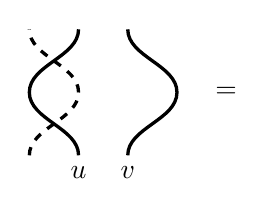
\begin{tikzpicture}[very thick,xscale=1.25 ,yscale=.8,baseline]
 \draw (1.5,-1) to[in=-90,out=90] node[below, at start]{$u$}
 (1,0) to[in=-90,out=90] (1.5,1) ; \draw[dashed] (1,-1)
 to[in=-90,out=90] (1.5,0) to[in=-90,out=90] (1,1); \draw
 (2,-1) to[in=-90,out=90] node[below, at start]{$v$} (2.5,0)
 to[in=-90,out=90] (2,1); 
\node at (3,0) {=}; 
 \end{tikzpicture}
 \begin{cases}
 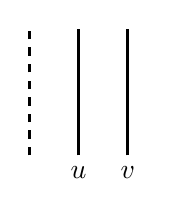
\begin{tikzpicture}[very thick,xscale=1.25 ,yscale=.8,baseline]
\draw (4.7,-1) --
 (4.7,1) node[below, at start]{$u$} ; \draw[dashed] (4.2,-1) to
 (4.2,1); \draw (5.2,-1) -- (5.2,1) node[below, at start]{$v$};
 \end{tikzpicture} & \text{for $u\neq qv$}\\
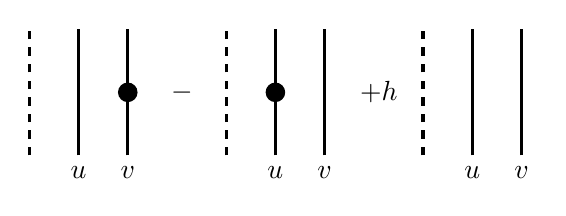
\begin{tikzpicture}[very thick,xscale=1.25,yscale=.8,baseline]
 \draw (4.7,-1) --
 (4.7,1) node[below, at start]{$u$} ; \draw[dashed] (4.2,-1) to
 (4.2,1); \draw (5.2,-1) -- (5.2,1) node[below, at start]{$v$}
 node[midway,fill,inner sep=2.5pt,circle]{}; \node at (5.75,0)
 {$-$};

 \draw (6.7,-1) -- (6.7,1) node[below, at start]{$u$}
 node[midway,fill,inner sep=2.5pt,circle]{}; \draw[dashed]
 (6.2,-1)-- (6.2,1); \draw (7.2,-1) -- (7.2,1) node[below, at
 start]{$v$};
\node at (7.75,0)
 {$+h$};
 \draw (8.7,-1) -- (8.7,1) node[below, at start]{$u$}; \draw[dashed]
 (8.2,-1)-- (8.2,1); \draw (9.2,-1) -- (9.2,1) node[below, at
 start]{$v$};
 \end{tikzpicture} & \text{for $u= qv$}
 \end{cases}
 \end{equation*} 
 \begin{equation*}\subeqn\label{triple-boring}
 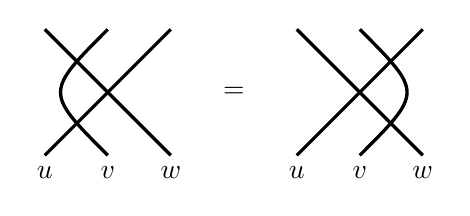
\begin{tikzpicture}[very thick,scale=1 ,scale=.8,baseline]
 \draw (-3,0) +(1,-1) -- +(-1,1) node[below,at start]{$w$}; \draw
 (-3,0) +(-1,-1) -- +(1,1) node[below,at start]{$u$}; \draw
 (-3,0) +(0,-1) .. controls (-4,0) .. +(0,1) node[below,at
 start]{$v$}; \node at (-1,0) {=}; \draw (1,0) +(1,-1) -- +(-1,1)
 node[below,at start]{$w$}; \draw (1,0) +(-1,-1) -- +(1,1)
 node[below,at start]{$u$}; \draw (1,0) +(0,-1) .. controls
 (2,0) .. +(0,1) node[below,at start]{$v$};
 \end{tikzpicture}
 \end{equation*}
 \begin{equation*}\subeqn \label{eq:triple-point1}
 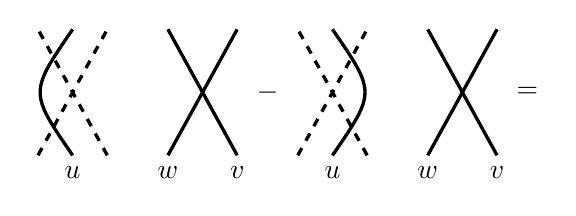
\begin{tikzpicture}[very thick,xscale=1.1,yscale=.8,baseline]
 \draw[dashed] (-3,0) +(.4,-1) -- +(-.4,1); \draw[dashed] (-3,0)
 +(-.4,-1) -- +(.4,1); \draw (-1.5,0) +(.4,-1) -- +(-.4,1)
 node[below,at start]{$v$}; \draw (-1.5,0) +(-.4,-1) -- +(.4,1)
 node[below,at start]{$w$}; \draw (-3,0) +(0,-1) .. controls
 (-3.5,0) .. +(0,1) node[below,at start]{$u$};\node at (-.75,0)
 {$-$}; \draw[dashed] (0,0) +(.4,-1) -- +(-.4,1); \draw[dashed]
 (0,0) +(-.4,-1) -- +(.4,1); \draw (1.5,0) +(.4,-1) -- +(-.4,1)
 node[below,at start]{$v$}; \draw (1.5,0) +(-.4,-1) -- +(.4,1)
 node[below,at start]{$w$}; \draw (0,0) +(0,-1) .. controls
 (.5,0) .. +(0,1) node[below,at start]{$u$}; \node at (2.25,0)
 {$=$}; 
 % \node[inner ysep=8pt,inner xsep=5pt,fill=white,draw,scale=.8]
 % at (6.2,0){$\displaystyle
 % \frac{Q_{ij}(y_3,y_2)-Q_{ij}(y_1,y_2)}{y_3-y_1}$};
 \end{tikzpicture}
 \begin{cases}
 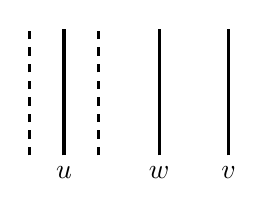
\begin{tikzpicture}[very thick,xscale=1.1,yscale=.8,baseline]
 \draw (4.5,0) +(.4,-1) -- +(.4,1) node[below,at
 start]{$v$}; \draw (4.5,0) +(-.4,-1) -- +(-.4,1) node[below,at
 start]{$w$}; \draw[dashed] (3,0) +(.4,-1) -- +(.4,1);
 \draw[dashed] (3,0) +(-.4,-1) -- +(-.4,1); \draw (3,0) +(0,-1)
 -- +(0,1) node[below,at start]{$u$};
 \end{tikzpicture}& \text{if $v=w=qu$}\\
 0 & \text{unless $v=w=qu$}
 \end{cases}
 \end{equation*}
\begin{equation*}\subeqn\label{eq:KLRtriple-point2}
 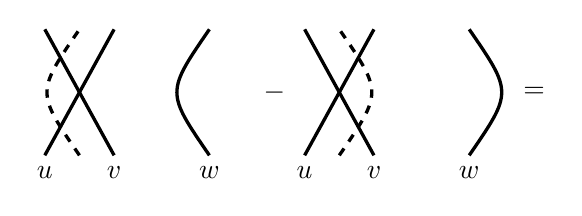
\begin{tikzpicture}[very thick,xscale=1.1,yscale=.8,baseline]
 \draw[dashed] (-3,0) +(0,-1) .. controls (-3.5,0) .. +(0,1) ;
 \draw (-3,0) +(.4,-1) -- +(-.4,1) node[below,at start]{$v$};
 \draw (-3,0) +(-.4,-1) -- +(.4,1) node[below,at start]{$u$};
 \draw (-1.5,0) +(0,-1) .. controls (-2,0) .. +(0,1)
 node[below,at start]{$w$};\node at (-.75,0) {$-$}; \draw (0,0)
 +(.4,-1) -- +(-.4,1) node[below,at start]{$v$}; \draw (0,0)
 +(-.4,-1) -- +(.4,1) node[below,at start]{$u$}; \draw[dashed]
 (0,0) +(0,-1) .. controls (.5,0) .. +(0,1); \draw (1.5,0)
 +(0,-1) .. controls (2,0) .. +(0,1) node[below,at
 start]{$w$}; \node at (2.25,0) {$=$}; \end{tikzpicture}
 \begin{cases}
 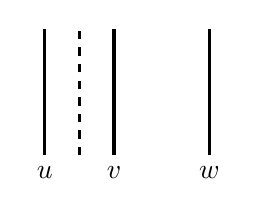
\begin{tikzpicture}[very thick,xscale=1.1,yscale=.8,baseline]\draw (3,0) +(.4,-1) --
 +(.4,1) node[below,at start]{$v$}; \draw (3,0) +(-.4,-1) --
 +(-.4,1) node[below,at start]{$u$}; \draw[dashed] (3,0) +(0,-1)
 -- +(0,1);\draw (4.5,0) +(0,-1) -- +(0,1) node[below,at
 start]{$w$};
 % \node[inner ysep=8pt,inner xsep=5pt,fill=white,draw,scale=.8]
 % at (6.2,0){$\displaystyle
 % \frac{Q_{ij}(y_3,y_2)-Q_{ij}(y_1,y_2)}{y_3-y_1}$};
 \end{tikzpicture}& \text{if $w =qu=qv$}\\
 0 & \text{unless $w\Mk =\Mk qu\Mk =\Mk qv$.}
 \end{cases}\mkern-9mu.
 \end{equation*}
\end{defi}
For the sake of completeness, here is an example of a weighted KLR
diagram:
\[
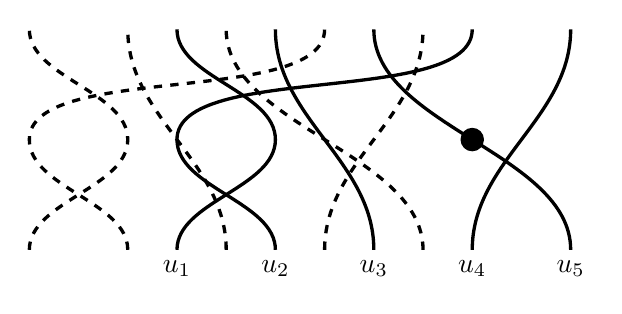
\begin{tikzpicture}[baseline,very thick,xscale=2.5,yscale=1.4]
 \draw (-.5,-1) to[out=90,in=-90] node[below,at start]{$u_2$} (-1,0) to[out=90,in=-90](.5,1);
 \draw[dashed] (-1.25,-1) to[out=90,in=-90] (-1.75,0) to[out=90,in=-90](-.25,1);
 \draw (.5,-1) to[out=90,in=-90]node[below,at start]{$u_4$} (1,1);
 \draw[dashed] (-.25,-1) to[out=90,in=-90] (.25,1);
 \draw (1,-1) to[out=90,in=-90] node[below,at start]{$u_5$}
 node[circle, midway,fill=black,inner sep=3pt]{} (0,1);
 \draw[dashed] (.25,-1) to[out=90,in=-90] (-.75,1);
 \draw (-1, -1) to[out=90,in=-90] node[below,at start]{$u_1$} (-.5,0) to[out=90,in=-90] (-1,1);
 \draw (0,-1) to[out=90,in=-90] node[below,at start]{$u_3$} (-.5,1);
 \draw[dashed] (-1.75, -1) to[out=90,in=-90] (-1.25,0) to[out=90,in=-90] (-1.75,1);
 \draw[dashed] (-.75,-1) to[out=90,in=-90] (-1.25,1);
\end{tikzpicture}\]
We can define a \emph{degree} function on KL diagrams, a special case
of the degree function in~\cite{WebwKLR}. The degrees are
given on elementary diagrams by 
\begin{equation}
 \deg\tikz[baseline,very thick,scale=1.5]{\draw (.2,.3) -- (-.2,-.1)
 node[at end,below,
 scale=.8]{$u$}; \draw (.2,-.1) -- (-.2,.3) node[at
 start,below,scale=.8]{$v$};}
 =-2 \qquad
 \deg\tikz[baseline,very thick,scale=1.5]{\draw (0,.3) -- (0,-.1)
 node[at
 end,below,scale=.8]{$u$} node[midway,circle,fill=black,inner
 sep=2pt]{};}=2
\qquad \deg\tikz[baseline,very thick,scale=1.5]{\draw (.2,.3) -- (-.2,-.1)
 node[at
 end,below,scale=.8]{$u$}; \draw[dashed] (.2,-.1) -- (-.2,.3)
 node[at
 start,below,scale=.8]{$v$};} = 
\deg\tikz[baseline,very
 thick,scale=1.5]{\draw[dashed] (.2,.3) -- (-.2,-.1) node[at
 end,below,scale=.8]{$u$}; \draw (.2,-.1) -- (-.2,.3) node[at
 start,below,scale=.8]{$v$};}
 =
\begin{cases}
 2 & u\Mk =\Mk qv\Mk =\Mk q^{-1}v\\
 1 & u\Mk =\Mk q^{\pm 1}v\Mk \neq \Mk q^{\mp 1}v\\
 0 & u\Mk \neq\Mk  q^{\pm 1}v
 \end{cases}\label{wKLR-grading}
\end{equation}
and $h$ is given grading $2$. Note that the relations
(\ref{dots-1}--\ref{eq:KLRtriple-point2}) are all homogeneous with wKLR diagrams given the
grading of~\eqref{wKLR-grading}.
\begin{prop}[{\cite[Prop.~2.7]{WebwKLR}}]\label{W-KLR-poly}
 The wKLR algebra $\gls{W}_{\mathscr{D}}(\pq)$ for a collection
 $\mathscr{D}$ has a faithful polynomial representation
 \[P_{\mathscr{D}} := \oplus_{D\in \mathscr{D}}\K[h,y_1,\dots,
 y_{|D|}]\]
defined by the rule that 
\begin{itemize}
\item Each crossing of the $r$ and $r+1$st strands acts by the Demazure operator \[\partial_r(f)=
 \frac{f^{s_r}-f}{y_{r+1}-y_{r}}.\]
\item 
A crossing between the $r$th strand and a ghost of $s$th strand acts
by
\begin{itemize}
\item the identity if $\ck <0$ and the
 strand is NE/SW or $\ck >0$ and the strand is NW/SE,
\item the multiplication operator of $y_s-y_r+h$ if $\ck <0$ and
 the strand is NW/SE or $\ck >0$ and the strand is NE/SW
\end{itemize}
\item A square on the $r$th strand acts by the multiplication operator
 $Y_r$. 
\end{itemize}
\end{prop}

Thus, we can again apply the results of Section~\ref{sec:polyn-style-repr},
with 
\begin{equation}
\mathbb{K}=\K[h]\qquad A=\gls{W}_{\mathscr{D}}(\pq) \qquad
 B=\K[h,y]\qquad I=B(h,y)\qquad P=P_{\mathscr{B}}.\label{eq:wKLR-PR}
\end{equation}

\begin{lemma}
 The polynomial representation $P_{\mathscr{D}}$ is graded polynomial-style
 with the data of~\eqref{eq:wKLR-PR}. 
\end{lemma}
\begin{proof}
\looseness-1 The algebra $\gls{W}_{\mathscr{D}}(\pq) $ is free over $B^{\otimes
 n}=\K[h,y_1,\dots, y_n]$ by~\cite[Thm.~2.8]{WebwKLR}, the
 centrality of $Z$ is clear from the relations and the faithfulness
 of $P$ follows from Proposition~\ref{W-KLR-poly}. The compatibility
 with grading is also clear from the definition
~\eqref{wKLR-grading}. 
\end{proof}

\begin{defi}\label{def:hW}
We let $\gls{hW}(h)$ be the completion of the weighted KLR algebra
$\gls{W}$ for $\gls{U}$
with respect to the grading; since $h$ has degree 2, this completion
is naturally a complete $\K\llbracket h\rrbracket $-module. For any collection $\mathscr{D}$, we let
$\gls{W}_{\mathscr{D}}(\pq),\gls{hW}_{\mathscr{D}}(\pq)$ be the sum of images of
the idempotents corresponding to loadings on a set of points in $\mathscr{D}$.
\end{defi} 

Let $\Bi$ be a loading in
the sense of~\cite{WebwKLR}, that is, a finite subset $D=\{d_1,\dots, d_n\}$ with
$d_1<\cdots <d_n$ of $\R$
together with a map $\Bi\colon D\to \gls{U}$.
In the algebra $\widehat{\waha}_{\mathscr{D}}(\pq)$, we have an idempotent
$\epsilon_{\Bi}$ projecting to the stable kernel of $X_j-\Bi(d_j)$
(that is, the kernel of a sufficiently large power). 
We represent $\epsilon_{\Bi}$ as a type W
diagram, with the strands labeled by the elements
$u_i=\Bi(d_j)$. 

\begin{theorem}\label{W-isomorphism}
 There is an isomorphism $\gamma\colon
 \widehat{\waha}_{\mathscr{D}}(\pq)\to \gls{hW}_{\mathscr{D}}(\pq)$ such
 that $\gamma(X_r)=\sum_{\Bu}u_rb({y_r})e_{\Bu}$,
\newseq
\[\subeqn\label{crossing-match}
\tikz[baseline,very thick,scale=1.5, green!50!black]{\draw (.2,.3) --
 (-.2,-.1); \draw
 (.2,-.1) -- (-.2,.3);} \epsilon_{\Bu}\mapsto
\begin{cases}
\displaystyle\frac{1}{u_{r+1}b(y_{r+1})-u_rb(y_{r})}(\psi_r-1) e_{\Bu} & u_r\neq u_{r+1}\\
 \displaystyle \frac{y_{r+1}-y_r}{u_{r+1}(b(y_{r+1})-b(y_{r}))}\psi_r e_{\Bu}& u_r=u_{r+1}
\end{cases}
\]
\[\subeqn\label{ghost-match}
\tikz[baseline,very thick,scale=1.5, green!50!black]{\draw[densely dashed] 
 (-.2,-.1)-- (.2,.3); \draw
 (.2,-.1) -- (-.2,.3);}\epsilon_{\Bu} \mapsto
\begin{cases}
\displaystyle u_rb(y_r)-\pq u_sb(y_s)\tikz[baseline,very thick,scale=1.5]{\draw[densely dashed]
 (-.2,-.1)-- (.2,.3); \draw
 (.2,-.1) -- (-.2,.3);} e_{\Bu}&
 u_r\neq qu_s\\ 
 \displaystyle \frac {u_rb(y_r)-\pq u_sb(y_s)}{y_{s}-y_{r}+d_1h}\tikz[baseline,very thick,scale=1.5]{\draw[densely dashed]
 (-.2,-.1)-- (.2,.3); \draw
 (.2,-.1) -- (-.2,.3);}e_{\Bu}& u_r=qu_s
\end{cases}
\qquad \qquad\tikz[baseline,very thick,scale=1.5, green!50!black]{\draw (.2,.3) --
 (-.2,-.1); \draw [densely dashed]
 (.2,-.1) -- (-.2,.3);} \mapsto \tikz[baseline,very thick,scale=1.5]{\draw (.2,.3) --
 (-.2,-.1); \draw [densely dashed]
 (.2,-.1) -- (-.2,.3);} \]
\end{theorem}
\begin{proof}
 This follows from comparing the polynomial representations. Exactly
 as argued in Lemma~\ref{lem:gammap}, the map is an isomorphism of
 vector spaces between the polynomial representations: the polynomial
 representation ${\cP}_{\mathscr{B}}$ has one copy of $\mathcal{C}$
 for each subset in $\mathscr{B}$. In $\widehat{\cP}_{\mathscr{B}}$,
 each of these copies is completed at $\gls{U}^n$, and becomes the direct
 sum of the images of $e_{\Bu}$, which is a copy of the completed
 polynomial ring. We can think of the choice of subset and of $\Bu$
 as giving a loading, which has a corresponding copy of $\widehat{C}$
 in $P_{\mathscr{B}}$. The map $\gamma_p$ induces an isomorphism
 between these completed polynomial rings.

 Now, we should
 consider how identifying completed polynomial representations via
 $\gamma_p$ affects how the basic diagrams of the WAHA act on the polynomial
 representation. 

 We have that \[\tikz[baseline,very thick,scale=1.5, green!50!black]{\draw (.2,.3) --
 (-.2,-.1); \draw
 (.2,-.1) -- (-.2,.3);} \cdot
f\epsilon_{\Bu}=\frac{f^{s_r}-f}{y_{r+1}-y_r}\epsilon_{\Bu}.
\]

If $u_r\neq u_{r+1}$, then $\psi_r\cdot
f\epsilon_\Bu=f^{s_r}\epsilon_\Bu$ and $u_{r+1}b(y_{r+1})-u_rb(y_r)$
is invertible, so the appropriate case of~\eqref{crossing-match} holds. If $u_r= u_{r+1}$, then
$\frac{u_{r}(b(y_{r+1})-b(y_r))}{y_{r+1}-y_r}$ is invertible, so the
formula is clear. 

Now, we turn to~\eqref{ghost-match}. We find that $\tikz[baseline,very thick,scale=1.5, green!50!black]{\draw[densely dashed] 
 (-.2,-.1)-- (.2,.3); \draw
 (.2,-.1) -- (-.2,.3);}\cdot f\epsilon_{\Bu}=(u_rb(y_r)-\pq u_sb(y_s) )f\epsilon_{\Bu}$. The first case of the isomorphism~\eqref{ghost-match} thus
follows directly from the polynomial representation of the wKLR algebra
given in Proposition~\ref{W-KLR-poly}. The second case of
\eqref{ghost-match} is clear.
\end{proof}





 The reader will note that the image of the idempotent $\gls{eprime}$ under
 this isomorphism is not homogeneous. On abstract grounds, there
 must exist a homogeneous idempotent $e''$ with isomorphic image. Let
 us give a description of one such, which is philosophically quite
 close to the approach of~\cite{SWschur}. 

Choose an arbitrary order
 on the elements of $\gls{U}$. The idempotent $e_\mu'$ for a composition
 $\mu$ is replaced by the sum of contributions from a list of
 multi-subsets $Z_i$ of $\gls{U}$ such that $|Z_i|=\mu_i$. There's a
 loading corresponding to these subsets, which we'll denote
 $\Bi_{Z_*}$. The underlying subset is $C_{\mu}$ as defined before;
 the points associated to the $j$th part at $x=js+\epsilon,\dots,
 js+\mu_j\epsilon$ are labeled with the elements of $Z_j$ in our
 fixed order. Finally, $e''_{Z_*}$ is the idempotent on this loading
 that acts on each group of strands with the same label in $\gls{U}$ and attached
 to the same part of $\mu$ with a fixed homogeneous primitive
 idempotent in the nilHecke algebra, for example, that acts as
$y^{k-1}_1\cdots y_{k-1}\partial_{w_0}$ in the polynomial
representation. Consider the sum $e''$ of the idempotents $e''_{Z_*}$ over all
$p$-tuples of multi-subsets. 

The idempotent $e''$ has
isomorphic image to $\gls{eprime}$, since $W\gls{eprime}'$ is a sum of projectives for
each composition $\mu$ whose
$(\mu_1!\cdots\mu_p!)$-fold direct sum is $We_{C_\mu}$.
Thus, the algebra $e''We''$ is graded and isomorphic to the Schur algebra.
It would be interesting to make this isomorphism a bit more
explicit, but we will leave that to other work. 

\section{Type F} 

\subsection{Type F Hecke algebras}
\label{sec:type-f-hecke}

Now let us turn to our other complication, analogous to that which
appeared in 
\cite{Webmerged}:
\begin{defi}
 A rank $n$ \emph{type F$_1$ Hecke diagram} is a rank $n$ affine Hecke diagram
 with a vertical red line inserted at $x=0$. The diagram must avoid
 tangencies and triple points with this strand as well, and only
 allow isotopies that preserve these conditions.
\end{defi}
We give an example of such a diagram below: 
\[
\begin{tikzpicture}[baseline,very thick,green!50!black, xscale=2,yscale=1.3]
 \draw (-.5,-1) to[out=90,in=-90] (-1,0) to[out=90,in=-90](.5,1);
 \draw (.5,-1) to[out=90,in=-90] (1,1);
 \draw[wei] (.25,-1) --(.25,1);
 \draw (1,-1) to[out=90,in=-90] 
 node[midway,fill=green!50!black,inner sep=3pt]{} (0,1);
 \draw (-1, -1) to[out=90,in=-90] (-.5,0) to[out=90,in=-90] (-1,1);
 \draw (0,-1) to[out=90,in=-90] (-.5,1);
\end{tikzpicture}\]

We decorate this red strand with a multisubset
$Q_\bullet=\{Q_1,\dots, Q_\ell\}\subset \gls{U}$ and let
$\PQ_i=Q_ie^{-z_i}$. To distinguish from other uses of the letter, we
let $\mathsf{e}_k(\Bz)$ be the degree $k$ elementary symmetric
function in an alphabet $\Bz$.
\begin{defi}
 Let the \emph{type F$_1$ affine Hecke algebra} $\tilde{\EuScript{F}} (\pq,\PQ_{\bullet})$ be the algebra generated over
 $\K\llbracket h,\Bz\rrbracket $ by type F$_1$ Hecke diagrams with $m$ strands modulo the
 local relations~\hbox{{\upshape (}\ref{qHecke-1}--\ref{qHecke-triple}{\upshape )}} and the
 local relations: \newseq
 \begin{equation*}\subeqn\label{qdumb}
 \begin{tikzpicture}[very thick,baseline=2.85cm,scale=.8]
 \draw[wei] (-3,3) +(1,-1) -- +(-1,1); \draw [green!50!black] (-3,3) +(0,-1)
 .. controls (-4,3) .. +(0,1); \draw [green!50!black] (-3,3) +(-1,-1) --
 +(1,1); \node at (-1,3) {=}; \draw[wei] (1,3) +(1,-1) --
 +(-1,1); \draw [green!50!black] (1,3) +(0,-1) .. controls (2,3) .. +(0,1);
 \draw [green!50!black] (1,3) +(-1,-1) -- +(1,1); \end{tikzpicture}
 \end{equation*}
 \begin{equation*}\subeqn\label{qred-dot}
 \begin{tikzpicture}[very thick,baseline,scale=.8]
 \draw [green!50!black](-3,0) +(-1,-1) -- +(1,1); \draw[wei](-3,0) +(1,-1) --
 +(-1,1); \node[ fill=green!50!black,inner
 sep=2.5pt] at (-3.5,-.5){}; \node at (-1,0) {=};
 \draw [green!50!black](1,0) +(-1,-1) -- +(1,1); \draw[wei](1,0) +(1,-1) --
 +(-1,1); \node[ fill=green!50!black,inner
 sep=2.5pt] at (1.5,.5){};
 \end{tikzpicture}
 \end{equation*}
 \begin{equation*}\label{qHcost}\subeqn
 \begin{tikzpicture}[very thick,baseline,scale=.7]
 \draw [wei] (-1.8,0) +(0,-1) -- +(0,1);
 \draw[green!50!black](-1.2,0) +(0,-1) .. controls (-2.8,0) ..
 +(0,1); \node at (-.3,0) {=}; \draw [green!50!black] (2.2,0)
 +(0,-1) -- node[midway, fill=green!50!black,inner
 sep=2.5pt,label=right:{$\ell$}]{}+(0,1); \draw[wei] (1.2,0)
 +(0,-1) -- +(0,1); \node at (4.3,0) {$+\,\mathsf{e}_1(-\PQ_\bullet)$};
 \draw[green!50!black] (6.8,0) +(0,-1) -- node[midway,
 fill=green!50!black,inner
 sep=2.5pt,label=right:{$\ell-1$}]{}+(0,1); \draw [wei] (5.8,0)
 +(0,-1) -- +(0,1); \node at (8.8,0) {$+$}; \node at (9.6,-.07)
 {$\cdots$}; \node at (11.35,0) {$+\mathsf{e}_{\ell}(-\PQ_\bullet)$};
 \draw[green!50!black] (13.8,0) +(0,-1) -- +(0,1); \draw [wei]
 (12.8,0) +(0,-1) -- +(0,1);
 \end{tikzpicture}
 \end{equation*}
 That is, on the RHS, we have the product $p_{\PQ}=(X_j-\PQ_1)\cdots
 (X_j-\PQ_\ell)$, where the green strand shown is the $j$th, and
 \begin{equation*}\label{qred-triple}\subeqn
 \begin{tikzpicture}[very thick,baseline=-2pt,scale=.7]
 \draw [wei] (0,-1) -- (0,1); \draw[green!50!black](.5,-1)
 to[out=90,in=-30] (-.5,1); \draw[green!50!black](-.5,-1)
 to[out=30,in=-90] (.5,1);
 \end{tikzpicture}- \begin{tikzpicture}[very
 thick,baseline=-2pt,scale=.7] \draw [wei] (0,-1) -- (0,1);
 \draw[green!50!black](.5,-1) to[out=150,in=-90] (-.5,1);
 \draw[green!50!black](-.5,-1) to[out=90,in=-150] (.5,1);
 \end{tikzpicture}
 =\sum_{i=1}^\ell\sum_{a+b=i-1}\mathsf{e}_{\ell-i}(-\PQ_\bullet)\cdot \Bigg(\begin{tikzpicture}[very thick,baseline=-2pt,scale=.7]
 \draw [wei] (0,-1) -- (0,1);
 \draw[green!50!black](.5,-1) to[out=90,in=-90] node[midway,
 fill=green!50!black,inner sep=2.5pt,label=right:{$b$}]{} (.5,1);
 \draw[green!50!black](-.5,-1) to[out=90,in=-90] node[midway,
 fill=green!50!black,inner sep=2.5pt,label=left:{$a+1$}]{} (-.5,1);
 \end{tikzpicture}-\pq \begin{tikzpicture}[very
 thick,baseline=-2pt,scale=.7] \draw [wei] (0,-1) -- (0,1);
 \draw[green!50!black](.5,-1) to[out=90,in=-90] node[midway,
 fill=green!50!black,inner sep=2.5pt,label=right:{$b+1$}]{}
 (.5,1); \draw[green!50!black](-.5,-1) to[out=90,in=-90]
 node[midway, fill=green!50!black,inner
 sep=2.5pt,label=left:{$a$}]{} (-.5,1);
 \end{tikzpicture}\Bigg).
 \end{equation*}
 The RHS can alternately by written as $(X_i-\pq
 X_{i+1})\frac{p_{\PQ}(X_i)-p_\PQ(X_{i+1})}{X_i-X_{i+1}}$.
\end{defi}
\begin{rema}
 As in the earlier cases, there is a degenerate version of this
 algebra, where we use the local relations
 (\ref{deg-Hecke-1}--\ref{deg-Hecke-triple}), leave (\ref{qdumb}--\ref{qHcost})
 unchanged, and replace the RHS of~\eqref{qred-triple} with $(X_i-
 X_{i+1}+1)\frac{p_{\PQ}(X_i)-p_\PQ(X_{i+1})}{X_i-X_{i+1}}$.
\end{rema}
We'll continue to use our convention of letting $X_r$ denote the sum
of all straight-line diagrams with a square on the $r$th green strand from
the left (ignoring red strands).

Given ${\mathscr{D}}$ a collection of subsets of $\R$, we'll let $\tilde{\EuScript{F}}_{\mathscr{D}}
(\pq,\PQ_{\bullet}),{\EuScript{F}}_{\mathscr{D}} (\pq,\PQ_{\bullet})$
denote the subalgebras of $\tilde{\EuScript{F}}
(\pq,\PQ_{\bullet}),{\EuScript{F}} (\pq,\PQ_{\bullet})$ spanned by
diagrams whose tops and bottoms lie in the set ${\mathscr{D}}$.


 Let $e_i$ be an arbitrarily fixed idempotent in $\tilde{\EuScript{F}} (\pq,\PQ_{\bullet})$ given by
 $i$ strands left of the red strand and $m-i$ right of it; let
 $\mathscr{D}^\circ$ be the collection of the corresponding
 sets. Since any idempotent is isomorphic to one of these by a
 straight-line diagram, enlarging $\mathscr{D}^\circ$ will give a
 Morita equivalent algebra. Let
 $\tilde{P}_n$ be the free $S[X_1^{\pm 1},\dots, X_n^{\pm 1}]$-module generated
 by elements $f_p$ for $p=0,\dots, m$.
\begin{prop}\label{tilde-poly}
 The algebra $\tilde{\EuScript{F}}_{\mathscr{D}^\circ} (\pq,\PQ_{\bullet})$ has a polynomial
 representation that sends
 \begin{itemize}
\item $e_i$ to the identity on the submodule generated by $f_i$.
\item $X_i$ to the multiplication operator and \[(T_i+1)\cdot
 F(X_1,\dots,X_n)f_p\mapsto (X_i-\pq X_{i+1})\frac{F^{s_i}-F}{X_{i+1}-X_i}f_p.\]
 \item the action of positive to negative crossing to the identity
 \[F(X_1,\dots,X_n)f_i\mapsto
 F(X_1,\dots,X_n)f_{i+1},\] and the opposite crossing to
 \[F(X_1,\dots,X_n)f_i\mapsto
 p_\PQ(X_i)F(X_1,\dots,X_n)f_{i-1}.\]
 \end{itemize}
\end{prop}
\begin{proof}
 This is a standard computation with Demazure operators.
\end{proof}


Now, we can allow several red
lines at various values of $x$, each of which carries a multiset of
values in $\gls{U}$. For the sake of notation, we'll still denote the
multiset given by all such labels as $\{Q_1,\dots, Q_\ell\}$, with a strand with the label
$Q_{i}$ at $x$-value
$\vartheta_i$. So, the situation we had previously considered was
$\vartheta_i=0$ for all $i$.

\begin{defi}\label{def:tF}
 A rank $n$ \emph{type F Hecke diagram} is a rank $n$ affine Hecke diagram
 with a vertical red lines inserted at $x=\vartheta_i$. The diagram must avoid
 tangencies and triple points with these strands as well, and only
 allow isotopies that preserve these conditions. We give an example
 of such a diagram below:
 \[
\begin{tikzpicture}[baseline,very thick,green!50!black, xscale=2,yscale=1.3]
 \draw (-.5,-1) to[out=90,in=-90] (-1,0) to[out=90,in=-90](.5,1);
 \draw (.5,-1) to[out=90,in=-90] (1,1);
 \draw (1,-1) to[out=90,in=-90] 
 node[midway,fill=green!50!black,inner sep=3pt]{} (0,1);
 \draw (-1, -1) to[out=90,in=-90] (-.5,0) to[out=90,in=-90] (-1,1);
 \draw (0,-1) to[out=90,in=-90] (-.5,1);
 \draw[wei](.25,-1) --(.25,1); \draw[wei](-.25,-1) --(-.25,1);
 \draw[wei](1.25,-1) --(1 .25,1);
\end{tikzpicture}\]

 Let the rank $n$ \emph{type F affine Hecke algebra} $\gls{tF}$ be the algebra generated over $\K\llbracket h,\Bz\rrbracket $ by
 rank $n$ type F Hecke diagrams for $\vartheta$ with $n$ strands modulo the
 local relations {\upshape (}\ref{qHecke-1}--\ref{qHecke-triple}{\upshape )} and
 {\upshape (}\ref{qdumb}--\ref{qred-triple}{\upshape )}.
\end{defi}
These algebras have a polynomial representation $\cP^{\vartheta}$ using the same maps
attached to basic diagrams as Proposition~\ref{tilde-poly}, but now
with idempotents, and thus copies of Laurent polynomials, indexed by weakly increasing
functions $\nu\colon [1,\ell]\to [0,m]$ with $\nu(i)$ giving the number of green strands to
the left of the $i$th red strand. This was carried out in more
detail in~\cite[Prop.~1.10]{MS18}. As before, any two idempotents
corresponding to $\nu$ are isomorphic by straight-line diagrams.

These affine type F algebras have ``finite-type'' quotients. In other
contexts, these have been called ``steadied'' or ``cyclotomic'' quotients.
\begin{defi}\label{def:cF}
 The rank $n$ \emph{type F Hecke algebra} $\gls{cF}$ is the quotient of $\gls{tF}$ by the 2-sided ideal generated by $e_{B}$ for
 every set $B$ possessing an element $b\in B$ with $b<\vartheta_i$
 for all $i$. 
\end{defi} 
Pictorially, the idempotents $e_B$ we kill possess a green strand
which is left of all the red strands. In~\cite{Webmerged}, the corresponding ideal for KLR
algebras is called the \emph{violating ideal} and we will use the same
terminology here. 
Given ${\mathscr{D}}$ a collection of subsets of $\R$, we'll let $\tilde{\EuScript{F}}^\vartheta_{\mathscr{D}}
(\pq,\PQ_{\bullet}),{\EuScript{F}}^\vartheta_{\mathscr{D}} (\pq,\PQ_{\bullet})$
denote the subalgebras of $\gls{tF},{\EuScript{F}}^\vartheta (\pq,\PQ_{\bullet})$ spanned by
diagrams whose tops and bottoms lie in the set ${\mathscr{D}}$.

\begin{prop}\label{prop:cyclo-Hecke}
 The rank $n$ cyclotomic affine Hecke algebra $\gls{cmH}(\pq,\PQ_\bullet)$ for the parameters $\{\PQ_1,\dots,
 \PQ_\ell\}$ is isomorphic to the rank $n$ type F$_1$ Hecke algebra
 $\EuScript{F}_{\mathscr{D}^\circ} (\pq,\PQ_{\bullet})$.
\end{prop}
\begin{proof}
 If we let $e$ be the idempotent given by green lines at $x=1,\dots, 
 n$, then we see by Theorem~\ref{wdHecke}, there is a map from the
 affine Hecke algebra sending $X_i$ and $T_i+1$ to diagrams as in
~\eqref{Hecke-gens} which induces a map
 $\iota\colon \gls{mH}(\pq)\to \EuScript{\tilde F}_{\mathscr{D}^\circ}
 (\pq,\PQ_{\bullet})$. 
Pulling back the polynomial representation of $\EuScript{\tilde F}_{\mathscr{D}^\circ}
 (\pq,\PQ_{\bullet})$ gives the polynomial representation of
 $\gls{mH}(\pq)$, which is faithful, so this map is injective.

 Applying 
~\eqref{qHcost} at the leftmost strand shows that $p_\PQ(X_1)$ lies
 in the violating ideal, which is the kernel of the map to
 $\EuScript{F}(\pq,\PQ_{\bullet})$. Thus, $\iota$ induces a
 map $\gls{cmH}(\pq,\PQ_\bullet)\to \EuScript{F}_{\mathscr{D}^\circ}
 (\pq,\PQ_{\bullet}). $ This map is clearly surjective, since any
 F$_1$ Hecke diagram with no violating strand is a composition of the
 images.
 
 Thus, we need only show that the preimage of
 the violating ideal under $\iota$ lies in the cyclotomic ideal. As in the proof of
~\cite[3.16]{Webmerged}, the relations (\ref{qHcost},\ref{qred-triple})
 allow us to reduce to the case where only a single green strand
 passes into the left half of the plane. In this case, we gain a
 factor of $p_\PQ(X_1)$, showing that this is in the cyclotomic
 ideal. 
\end{proof}

\subsection{Stendhal algebras}
\label{sec:stendhal-algebras}


The type F algebras in the KLR family have been introduced in
\cite{Webmerged}. 
Let $o_1=\min(\vartheta_i)$, and
$o_j=\min_{\vartheta_i>o_{j-1}}(\vartheta_i)$; so these are the real
numbers that occur as $\vartheta_i$ in increasing order.
Consider the sequence $\la_j=\sum_{\vartheta_i=o_j}\omega_{Q_i}$ of
dominant weights for $\mathfrak{g}_{\gls{U}}$, and let $S_{u,j}=\{s\in
[1,\ell]|\vartheta_s=o_j, u=Q_s\}$.

In
\cite[Def.~4.7]{Webmerged}, we defined algebras
$T^\bla,\tilde{T}^\bla$ attached to this list of weights. These
cannot match $\gls{htF},\gls{cF}$ since they are not naturally modules over
 $\K\llbracket h,\Bz\rrbracket $; however, we will recover them when we set
 $h=z_1=\cdots=z_\ell=0$. Instead, we should consider deformed
 versions of these algebras $\tilde{T}^\bla(h,\Bz),T^\bla(h,\Bz)$
 introduced in~\cite[\S~3.2]{WebwKLR} based on
 the canonical deformation of weighted KLR algebras. As usual, we'll
 let $y_r$ denote the sum of all straight line Stendhal diagrams with
 a dot on the $r$th strand.
 \begin{defi}\label{def:tT}
 We let the rank $n$ affine Stendhal algebra $\gls{tT}$ be the quotient of the algebra
 freely spanned over $\K[h,\Bz]$ by Stendhal diagrams (as defined
 in~\cite[\S~3.2]{Webmerged}) with $n$
 black strands, with the local
 relations {\upshape (}\ref{first-QH}--\ref{triple-dumb}{\upshape )} and the
 local relations\newseq
 \begin{equation*}\label{cost}\subeqn
 \begin{tikzpicture}[very thick,scale=.8,baseline=1.2cm]
 \draw (-2.8,0) +(0,-1) .. controls (-1.2,0) .. +(0,1)
 node[below,at start]{$u$}; \draw[wei] (-1.2,0) +(0,-1)
 .. controls (-2.8,0) .. +(0,1) node[below,at
 start]{$\la_j$}; \node at (-.3,0) {$=p_{u,j}$};
 \node[scale=1.5] at (.5,0) {$\Bigg($}; \node[scale=1.5] at
 (3.5,0) {$\Bigg)$}; \draw[wei] (2.8,0) +(0,-1) -- +(0,1)
 node[below,at start]{$\la_j$}; \draw (1.2,0) +(0,-1) -- +(0,1)
 node[below,at start]{$u$}; \fill (1.2,0) circle (3pt);
 \draw[wei] (-2.8,3) +(0,-1) .. controls (-1.2,3) .. +(0,1)
 node[below,at start]{$\la_j$}; \draw (-1.2,3) +(0,-1)
 .. controls (-2.8,3) .. +(0,1) node[below,at start]{$u$};
 \node at (-.3,3) {$=p_{u,j}$};\node[scale=1.5] at (.5,3)
 {$\Bigg($}; \node[scale=1.5] at (3.5,3) {$\Bigg)$}; \draw
 (2.8,3) +(0,-1) -- +(0,1) node[below,at start]{$u$};
 \draw[wei] (1.2,3) +(0,-1) -- +(0,1) node[below,at
 start]{$\la_j$}; \fill (2.8,3) circle (3pt);
 \end{tikzpicture}\qquad
 p_{u,j}(y)=\prod_{s\in S_{u,j}}(y-z_{s})
 \end{equation*}
 \begin{equation*}\subeqn\label{dumb}
 \begin{tikzpicture}[very thick,baseline=2.85cm,scale=.8]
 \draw[wei] (-3,3) +(1,-1) -- +(-1,1); \draw (-3,3) +(0,-1)
 .. controls (-4,3) .. +(0,1); \draw (-3,3) +(-1,-1) --
 +(1,1); \node at (-1,3) {=}; \draw[wei] (1,3) +(1,-1) --
 +(-1,1); \draw (1,3) +(0,-1) .. controls (2,3) .. +(0,1);
 \draw (1,3) +(-1,-1) -- +(1,1); \end{tikzpicture}
 \end{equation*}
 \begin{equation*}\subeqn\label{red-dot}
 \begin{tikzpicture}[very thick,baseline,scale=.8]
 \draw(-3,0) +(-1,-1) -- +(1,1); \draw[wei](-3,0) +(1,-1) --
 +(-1,1); \fill (-3.5,-.5) circle (3pt); \node at (-1,0) {=};
 \draw(1,0) +(-1,-1) -- +(1,1); \draw[wei](1,0) +(1,-1) --
 +(-1,1); \fill (1.5,.5) circle (3pt);
 \end{tikzpicture}
 \end{equation*}
\begin{equation*}\label{red-triple}\subeqn
 \begin{tikzpicture}[very thick,baseline=-2pt,scale=.8]
 \draw [wei] (0,-1) -- node[below,at start]{$\la_j$} (0,1);
 \draw(.5,-1) to[out=90,in=-30] node[below,at start]{$u$}
 (-.5,1); \draw(-.5,-1) to[out=30,in=-90] node[below,at
 start]{$v$} (.5,1);
 \end{tikzpicture}- \begin{tikzpicture}[very thick,baseline=-2pt,scale=.8]
 \draw [wei] (0,-1) --node[below,at start]{$\la_j$} (0,1);
 \draw(.5,-1) to[out=150,in=-90] node[below,at start]{$u$}
 (-.5,1); \draw(-.5,-1) to[out=90,in=-150] node[below,at
 start]{$v$} (.5,1);
 \end{tikzpicture}
\Mk  = \Mk \delta_{u,v}\sum_{p\Mk =\Mk 1}^{\al_u^\vee(\la_j)}\sum_{a\Mk +\Mk b\Mk =\Mk p\Mk -\Mk 1}\mathsf{e}_{\al_i^\vee(\la_j)-p}\big(\{-z_s\mid
 s\in S_{u,j}\}\big) \cdot \Bigg(\begin{tikzpicture}[very thick,baseline=-2pt,scale=.8]
 \draw [wei] (0,-1) -- (0,1);
 \draw(.5,-1) to[out=90,in=-90] node[midway,circle,
 fill=black,inner sep=2pt,label=right:{$b$}]{} (.5,1);
 \draw(-.5,-1) to[out=90,in=-90] node[midway,circle,
 fill=black,inner sep=2pt,label=left:{$a$}]{} (-.5,1);
 \end{tikzpicture}\Bigg).
 \end{equation*}
 The rank $n$ Stendhal algebra $\gls{cT}$ is the quotient of
 $\gls{tT}$ by violating diagrams as defined in
~\cite[Def.~4.3]{Webmerged}.
 \end{defi}
 Again for the sake of comparison, here is an example of a Stendhal
 diagram of rank~5: 
 \[
\begin{tikzpicture}[baseline,very thick,xscale=2,yscale=1.3]
 \draw (-.5,-1) to[out=90,in=-90] node[below,at start]{$u_2$} (-1,0) to[out=90,in=-90](.5,1);
 \draw (.5,-1) to[out=90,in=-90] node[below,at start]{$u_4$} (1,1);
 \draw (1,-1) to[out=90,in=-90] node[below,at start]{$u_5$}
 node[circle, midway,fill=black,inner sep=3pt]{} (0,1);
 \draw (-1, -1) to[out=90,in=-90]node[below,at start]{$u_1$} (-.5,0) to[out=90,in=-90] (-1,1);
 \draw (0,-1) to[out=90,in=-90] node[below,at start]{$u_3$} (-.5,1);
 \draw[wei](.25,-1) -- node[below,at start]{$\la_2$} (.25,1); \draw[wei](-.25,-1) --node[below,at start]{$\la_1$} (-.25,1);
 \draw[wei](1.25,-1) --node[below,at start]{$\la_3$} (1 .25,1);
\end{tikzpicture}\] 
This algebra is graded with Stendhal diagrams given their usual
grading, summing local contributions given by 
\[
 \deg\tikz[baseline,very thick,scale=1.5]{\draw (.2,.3) --
 (-.2,-.1) node[at end,below, scale=.8]{$u$}; \draw (.2,-.1) --
 (-.2,.3) node[at start,below,scale=.8]{$v$};}
 =-\langle\al_u,\al_v\rangle \qquad \deg\tikz[baseline,very
 thick,scale=1.5]{\draw (0,.3) -- (0,-.1) node[at
 end,below,scale=.8]{$u$} node[midway,circle,fill=black,inner
 sep=2pt]{};}=2 \qquad
 \deg\tikz[baseline,very thick,scale=1.5]{\draw[wei] (.2,.3) --
 (-.2,-.1) node[at end,below, scale=.8]{$\la$}; \draw (.2,-.1) --
 (-.2,.3) node[at start,below,scale=.8]{$u$};}
 =\deg\tikz[baseline,very thick,scale=1.5]{\draw (.2,.3) --
 (-.2,-.1) node[at end,below, scale=.8]{$u$}; \draw[wei] (.2,-.1) --
 (-.2,.3) node[at start,below,scale=.8]{$\la$};}=\al_u^{\vee}(\la),\]
and the variables $h$ and $z_i$ each have degree 2.

 The algebra $\gls{tT}$ has a polynomial representation $P_{\bla}$, given in
~\cite[Lem.~4.12]{Webmerged}. In order to match the Hecke side,
 we will use the version of this representation that has
 \[P_{uv}(a,b)=
 \begin{cases}
 b-a+h & u=qv\\
1 & u\neq qv.
 \end{cases}
 \] 

For every loading, we have an associated function $\kappa$, with
$\kappa(k)$ equal to
the number of black strands to the left of $o_k$, and a sequence
$(u_1,\dots, u_n)$ given by the eigenvalues we've attached to each
black strand. We let $e_{\Bu,\kappa}$ be the idempotent associated to this
data in $\gls{tT}$ and by extension in
$\gls{htT}$ and $\gls{cT}$.

\subsection{Isomorphisms}
\label{sec:isomorphisms}

As in types O and W, these algebras have polynomial-style
representations (graded in the case of $\gls{tT}$, with the data
\begin{gather*}%\notag
\mathbb{K}=\K\llbracket h\rrbracket \quad A=\gls{tF}\quad
 B=\K\llbracket h\rrbracket [X^{\pm}]\quad I=Bh+B\prod_{u\in \gls{U}}(X-u)\quad P=\cP_{\theta}%\label{eq:fHecke-PR}
\\
\mathbb{K}=\K[h]\quad A=\gls{tT} \quad
 B=\K[h,y]\quad I=Bh+By \quad P=P_{\bla}.%\label{eq:fKLR-PR}
\end{gather*}
and the polynomial representations we have defined, with the latter
being graded. This is proven exactly as in the earlier cases:
\begin{enumerate}
\item An explicit basis indexed by permutations, constructed for
 $\gls{tF}$ in~\cite[Prop.~1.15]{MS18} and $\gls{tT} $ in
~\cite[Prop.~4.16]{Webmerged}, shows the required freeness.
 \item The
 centrality of $Z$ is immediate from the relations.
 \item The
 faithfulness of the representations is checked in
~\cite[Prop.~1.11]{MS18} and implicit in the proof of
~\cite[Prop.~4.16]{Webmerged}, respectively.
\end{enumerate}



 We let $\gls{htF}$ and 
 $\gls{htT}$ be the completions of these rings with respect to the
 induced topology. Since $h$ and $\Bz$ both have positive
 degree, $\gls{htT}$ is a complete module over $\K\llbracket h,\Bz\rrbracket $.

\begin{theorem}\label{F-isomorphism}
 We have an isomorphism $\gls{htF}\cong \gls{htT}$ which induces an
 isomorphism $\gls{cF}\cong \gls{cT}$, given by 
\[\epsilon_{\Bu,\kappa}\mapsto e_{\Bu,\kappa}\qquad\qquad X_r\mapsto\sum_{\Bu,\kappa}u_rb({y_r})e_{\Bu,\kappa}\qquad \qquad \tikz[baseline,very thick,scale=1.5, green!50!black]{\draw [wei] (.2,.3) --
 (-.2,-.1); \draw 
 (.2,-.1) -- (-.2,.3);} \mapsto\tikz[baseline,very
 thick,scale=1.5]{\draw [wei] (.2,.3) -- (-.2,-.1); \draw (.2,-.1) --
 (-.2,.3);}\]
 \vspace{-3mm}

\[\tikz[baseline,very thick,scale=1.5, green!50!black]{\draw [wei] (-.2,.3) --
 (.2,-.1); \draw 
 (-.2,-.1) -- (.2,.3);} \epsilon_{\Bu,\kappa} \mapsto
\frac{\displaystyle\prod_{\vartheta_s=o_k}(u_rb({y_r-z_s})-\PQ_s)}{\displaystyle\prod_{s\in
 S_{u_r,j}} (y_r-z_s)}\, \tikz[baseline,very thick,scale=1.5]{\draw [wei] (-.2,.3) --
 (.2,-.1); \draw 
 (-.2,-.1) -- (.2,.3);} e_{\Bu,\kappa} 
\qquad \qquad \tikz[baseline,very thick,scale=1.5, green!50!black]{\draw (.2,.3) --
 (-.2,-.1); \draw
 (.2,-.1) -- (-.2,.3);}\, e_{\Bu,\kappa}\mapsto
A_r^{\Bu}\tikz[baseline,very thick,scale=1.5]{\draw (.2,.3) --
 (-.2,-.1); \draw
 (.2,-.1) -- (-.2,.3);} e_{\Bu,\kappa} \]
where the leftmost green/black strand shown is the $r$th from the
left, and the red strand shown is the $j$th from the left.
\end{theorem}
\begin{proof}
 Since all generators and relations involve at most one red line, we
 can assume that $\ell=1$, and use the representation of Proposition
~\ref{tilde-poly} for the Hecke side. That diagrams with only green
 strands have actions that match is just Theorem~\ref{O-isomorphism}.
 Thus, we only need to check the crossing of green and red strands is
 intertwined with a crossing of red and black strands. Since we have
 only one red strand, we have that
 $\prod_{\vartheta_s=o_k}(u_re^{y_r}-\PQ_s)=p_{\PQ_\bullet}(u_re^{y_r})$.
 Thus, comparing the representation of Proposition~\ref{tilde-poly} with
 the obvious $\K[h,\Bz]$-deformation of the action in
~\cite[Lem.~4.12]{Webmerged} yields the result.
\end{proof}

\section{Type WF}
\label{sec:antigens-ab}

\subsection{Type WF Hecke algebras}

Finally, we consider these two complications jointly. As mentioned
before, these are unlikely to be familiar algebras for the reader, but 
these results will ultimately be
useful in understanding category $\cO$ of rational Cherednik algebras
in~\cite{WebRou}. 
\begin{defi}\label{def:tWF}
 A rank $n$ \emph{type WF Hecke diagram} is a type W Hecke diagram
 with vertical red lines inserted at $x=\vartheta_i$. The diagram must avoid
 tangencies and triple points between any combination of these
 strands, green strands and ghosts, and only
 allow isotopies that preserve these conditions. An example of a rank 5 type WF diagram with $g<0$ is given below:
\[
\begin{tikzpicture}[baseline,very thick,green!50!black, xscale=2.5,yscale=1.4]
 \draw (-.5,-1) to[out=90,in=-90] (-1,0) to[out=90,in=-90](.5,1);
 \draw[dashed] (-1.25,-1) to[out=90,in=-90] (-1.75,0) to[out=90,in=-90](-.25,1);
 \draw (.5,-1) to[out=90,in=-90] (1,1);
 \draw[dashed] (-.25,-1) to[out=90,in=-90] (.25,1);
 \draw (1,-1) to[out=90,in=-90] 
 node[midway,fill=green!50!black,inner sep=3pt]{} (0,1);
 \draw[dashed] (.25,-1) to[out=90,in=-90] (-.75,1);
 \draw (-1, -1) to[out=90,in=-90] (-.5,0) to[out=90,in=-90] (-1,1);
 \draw (0,-1) to[out=90,in=-90] (-.5,1);
 \draw[dashed] (-1.75, -1) to[out=90,in=-90] (-1.25,0) to[out=90,in=-90] (-1.75,1);
 \draw[dashed] (-.75,-1) to[out=90,in=-90] (-1.25,1);
 \draw[wei](.125,-1) --(.125,1); \draw[wei](-.9,-1) --(-.9,1);
 \draw[wei](1.125,-1) --(1.125,1);
\end{tikzpicture}\]

Let the rank $n$ \emph{type WF affine Hecke algebra} $\gls{tWF}^\vartheta (\pq,\PQ_{\bullet})$ be the 
$\K\llbracket h,\Bz\rrbracket $-algebra generated by
 type WF Hecke diagrams modulo the local relations
 {\upshape (}\ref{nilHecke-2}--\ref{eq:triple-point-2},~\ref{qdumb}--\ref{qHcost}{\upshape )} and \newseq
 \begin{equation*}\label{PCsmart-red-triple}\subeqn
 \begin{tikzpicture}[very thick,baseline=-2pt,scale=.7]
 \draw [wei] (0,-1) -- (0,1); \draw[green!50!black](.5,-1)
 to[out=90,in=-30] (-.5,1); \draw[green!50!black](-.5,-1)
 to[out=30,in=-90] (.5,1);
 \end{tikzpicture}- \begin{tikzpicture}[very
 thick,baseline=-2pt,scale=.7] \draw [wei] (0,-1) -- (0,1);
 \draw[green!50!black](.5,-1) to[out=150,in=-90] (-.5,1);
 \draw[green!50!black](-.5,-1) to[out=90,in=-150] (.5,1);
 \end{tikzpicture}
 =\sum_{i=1}^\ell\sum_{a+b=i-1}\mathsf{e}_{\ell-i}(-\PQ_\bullet)\cdot \Bigg(\begin{tikzpicture}[very thick,baseline=-2pt,scale=.7]
 \draw [wei] (0,-1) -- (0,1);
 \draw[green!50!black](.5,-1) to[out=90,in=-90] node[midway,
 fill=green!50!black,inner sep=2.5pt,label=right:{$b$}]{} (.5,1);
 \draw[green!50!black](-.5,-1) to[out=90,in=-90] node[midway,
 fill=green!50!black,inner sep=2.5pt,label=left:{$a$}]{} (-.5,1);
 \end{tikzpicture}\Bigg).
 \end{equation*}
 \begin{equation*}\label{PC-dumb-red-triple}\subeqn
 \begin{tikzpicture}[very thick,baseline=-2pt,yscale=.8,]
 \draw [wei] (0,-1) -- (0,1);
 \draw[green!50!black,dashed](.5,-1) to[out=90,in=-30] (-.5,1);
 \draw[green!50!black](-.5,-1) to[out=30,in=-90] (.5,1);
 \end{tikzpicture}= \begin{tikzpicture}[very thick,baseline=-2pt,yscale=.8,]
 \draw [wei] (0,-1) -- (0,1);
 \draw[green!50!black,dashed](.5,-1) to[out=150,in=-90] (-.5,1);
 \draw[green!50!black](-.5,-1) to[out=90,in=-150] (.5,1);
 \end{tikzpicture}\qquad \qquad \begin{tikzpicture}[very thick,baseline=-2pt,yscale=.8,]
 \draw [wei] (0,-1) -- (0,1);
 \draw[green!50!black](.5,-1) to[out=90,in=-30] (-.5,1);
 \draw[green!50!black,dashed](-.5,-1) to[out=30,in=-90] (.5,1);
 \end{tikzpicture}= \begin{tikzpicture}[very thick,baseline=-2pt,yscale=.8]
 \draw [wei] (0,-1) -- (0,1);
 \draw[green!50!black](.5,-1) to[out=150,in=-90] (-.5,1);
 \draw[green!50!black,dashed](-.5,-1) to[out=90,in=-150] (.5,1);
 \end{tikzpicture}\qquad \qquad \begin{tikzpicture}[very thick,yscale=.8,baseline=-2pt]
 \draw [wei] (0,-1) -- (0,1);
 \draw[green!50!black,dashed](.5,-1) to[out=90,in=-30] (-.5,1);
 \draw[green!50!black,dashed](-.5,-1) to[out=30,in=-90] (.5,1);
 \end{tikzpicture}= \begin{tikzpicture}[very thick,yscale=.8,baseline=-2pt]
 \draw [wei] (0,-1) -- (0,1);
 \draw[green!50!black,dashed](.5,-1) to[out=150,in=-90] (-.5,1);
 \draw[green!50!black,dashed](-.5,-1) to[out=90,in=-150] (.5,1);
 \end{tikzpicture}
\end{equation*}
\end{defi}
\begin{rema}
 The degenerate version of this algebra is defined by the local relations
 (\ref{nilHecke-2}--\ref{NilHecke3},~\ref{eq:triple-point-2}--\ref{eq:deg-triple-point-1},
~\ref{qdumb}--\ref{qHcost},~\ref{PCsmart-red-triple}--\ref{PC-dumb-red-triple})
\end{rema}
Note that relation~\eqref{qred-triple} is \emph{not} true in this
algebra. As before, we should think of type F diagrams as type WF
diagrams with $\ck$ so small that we cannot see that the ghost and
strand are separate. Using this approach, we can see that relation
\eqref{qred-triple} for a strand and a ghost together is a consequence
of~\eqref{ghost-bigon1} and~\eqref{PCsmart-red-triple}, much as in
Theorem~\ref{wdHecke}.

This algebra has a polynomial representation $P^\vartheta$, defined
using the same formulae as those of Propositions~\ref{W-poly} and
\ref{tilde-poly}. We leave the routine computations that these are compatible
with~\eqref{PCsmart-red-triple} and~\eqref{PC-dumb-red-triple} to the reader.

We call an idempotent \emph{unsteady} if the strands can be
divided into two groups with a gap $>|\ck|$ between them
and all red strands in the right hand group, and \emph{steady} otherwise. 

Thus, the idempotents shown in~\eqref{steady} are steady, and those in
\eqref{unsteady} are unsteady.
\newseq
\[\subeqn\label{steady}\tikz[baseline=-2pt,very thick, xscale=3,green!50!black] { 
\draw (.05,-.5) -- (0.05,.5);
\draw[dashed] (-.55,-.5) -- (-.55,.5);
\draw[dashed] (-.1,-.5) -- (-.1,.5);
\draw (.5,-.5) -- (.5,.5);
\draw[wei](.35,-.5) -- (.35,.5);
 }
 \hspace{3cm} \tikz[baseline=-2pt,very thick, xscale=3,green!50!black] { 
\draw (1.25,-.5) -- (1.25,.5);
\draw[dashed] (.65,-.5) -- (.65,.5);
\draw[dashed] (-.1,-.5) -- (-.1,.5);
\draw (.5,-.5) -- (.5,.5);
\draw[wei](.35,-.5) -- (.35,.5);
 }\]
\[\subeqn\label{unsteady}\tikz[baseline=-2pt,very thick, xscale=3,green!50!black] { 
\draw (-.25,-.5) -- (-0.25,.5);
\draw[dashed] (-.85,-.5) -- (-.85,.5);
\draw[dashed] (-.1,-.5) -- (-.1,.5);
\draw (.5,-.5) -- (.5,.5);
\draw[wei](.35,-.5) -- (.35,.5);
 } \hspace{3cm}\tikz[baseline=-2pt,very thick, xscale=3,green!50!black] { 
\draw (-.25,-.5) -- (-0.25,.5);
\draw[dashed] (-.85,-.5) -- (-.85,.5);
\draw[dashed] (-.4,-.5) -- (-.4,.5);
\draw (.2,-.5) -- (.2,.5);
\draw[wei](.35,-.5) -- (.35,.5);
 }\]


 \begin{defi}\label{def:cWF} 
 Let the rank $n$ \emph{type WF Hecke algebra}
 $\gls{cWF}^\vartheta (\pq,\PQ_{\bullet})\cong \PC^\vartheta$
 be the quotient of
 $\gls{tWF}^\vartheta (\pq,\PQ_{\bullet})$ by the
 ideal generated by all unsteady idempotents.
 \end{defi}


We can also call this a ``pictorial
 Cherednik algebra,'' referring to the fact that the representation
 category of this algebra when $\K=\Cbb$ and we set $h=z_i=0$ is
 equivalent to the category
 $\cO$ over a Cherednik algebra for the group $\Z/\ell\Z\wr S_n$ for
 certain parameters. More precisely, we consider the category $\cO$ over the
 rational Cherednik algebra $\mathsf{H}$ for the group $\Z/\ell\Z\wr
 S_n$ with arbitrary $\Cbb$-valued parameters $k,
 s_1,\dots, s_\ell$, using the conventions of~\cite[\S~2.1]{WebRou}
 and consider the algebra
 $\gls{cWF}^\vartheta (\pq,\PQ_{\bullet})$ where fix the
 number of green strands to be $n$, and fix the parameters $g=\Rerm(k),
 \vartheta_p=\Rerm(ks_p), q\expe^{2\pi \ir k}$, and $Q_p=\expe^{2\pi \ir k s_p}$.
 \begin{theorem}[{\cite[Cor.~3.10]{WebRou}}]
 For the parameters discussed above, we have an equivalence of
 categories $\cO\cong
 \gls{cWF}^\vartheta (\pq,\PQ_{\bullet})\mmod$. 
\end{theorem}
Obviously, any choice of $q,Q_\bullet$ can be realized this way for
some $k,s_\bullet$, which are not unique; for any $g$ and $\vartheta$,
we can adjust the choice of parameters $ k,s_\bullet$ to yield an
block of the Cherednik category $\cO$ that matches the representations
of $\gls{cWF}^\vartheta (\pq,\PQ_{\bullet})$, using the process
of Uglovation discussed in~\cite[Def.~2.8]{WebRou}.
 This is also useful to consider as a common generalization of all
 the algebras we have considered. 
Given a collection ${\mathscr{D}}$ of subsets of $\R$, we'll let $\gls{tWF}^\vartheta_{\mathscr{D}}
(\pq,\PQ_{\bullet}),\gls{cWF}_{\mathscr{D}}^\vartheta (\pq,\PQ_{\bullet})$
denote the subalgebras of $\gls{tWF}^\vartheta
(\pq,\PQ_{\bullet}), \gls{cWF}^\vartheta (\pq,\PQ_{\bullet})$ spanned by
diagrams whose tops and bottoms lie in the set ${\mathscr{D}}$. 

As in earlier cases, the algebra $\gls{tWF}^\vartheta (\pq,\PQ_{\bullet})$
 is equipped with a polynomial representation $P^\vartheta$ using the rules of
 Proposition~\ref{W-poly} for diagrams only involving green strands and
 Proposition~\ref{tilde-poly} for basic diagrams involving red and
 green strands.

 \subsubsection{Relation to cyclotomic Schur algebras}
\label{sec:relation-hecke-schur}


We can extend Theorem~\ref{wdHecke} to this setting. As before, let
$\wellsep=\{B_s=\{s,2s,3s,\dots, ns\}\}$ for $s$ some real
number with $s\gg |\ck|,|\vartheta_i|$. 
\begin{theorem}\label{wfHecke}
 There is an isomorphism of $\gls{cWF}^\vartheta_\wellsep
 (\pq,\PQ_{\bullet})$ to the rank $n$ cyclotomic affine Hecke algebra
 $\gls{cmH}(\pq,\PQ_\bullet)$ for the 
 parameters $\{\PQ_1,\dots, \PQ_\ell\}$. 
\end{theorem}
\begin{proof}
 First, since $s\gg |\vartheta_i|$, all strands start and end to the
 right of all red strands. Thus, we have that every diagram can be
 written, using the relations, in terms of diagrams that remain to
 the right of all red strands. Thus, we have a surjective map from
 the type W affine Hecke algebra $\waha_\cO$ onto $\gls{cWF}^\vartheta_\wellsep
 (\pq,\PQ_{\bullet})$. 
By Theorem~\ref{wdHecke}, we can identify $\waha_\cO$ with the usual
affine Hecke algebra $\hmH$. 

Now consider a diagram
where the first strand starts at $(s,0)$, goes linearly to
$(-s,\nicefrac 12)$ then back to $(s,1)$, while all others remain
straight. This diagram is unsteadied, since the horizontal slice at
$y=\nicefrac{1}2$ is unsteadied by the leftmost strand. By the relation~\eqref{qHcost}, this diagram is equal to $\prod_{i=1}^\ell
 (X_1-\PQ_i)$ which thus lies in the kernel of the map of the affine
 Hecke algebra to $\gls{cWF}^\vartheta_\wellsep
 (\pq,\PQ_{\bullet})$. 

 As in the proof of~\ref{prop:cyclo-Hecke}, we can easily check that
 the diagram discussed above generates the kernel so $\gls{cWF}^\vartheta_\wellsep (\pq,\PQ_{\bullet})$ is isomorphic to
 this cyclotomic quotient.
\end{proof}

There is also a version of this theorem relating the type WF Hecke
algebras to cyclotomic Schur algebras. Assume that the parameters
$\vartheta_i$ are ordered with $\vartheta_1<\dots <\vartheta_\ell$.
Fix a set $\Lambda$ of $\ell$-multicompositions of $n$ which is an
upper order ideal in dominance order. We'll be interested in the
cyclotomic $q$-Schur algebra $\gls{cycSchur}$ of rank $n$ attached to the
data $(\pq,\PQ^\bullet)$ defined by Dipper, James and Mathas
\cite[6.1]{DJM}; let $ \glslink{cycSchur}{\mathscr{S}^-(\Lambda)}$ be the signed version of
this algebra defined using signed permutation modules.

Let $r$ be
the maximum number of parts of one of the components of $\xi\in
\Lambda$. Choose constants $\epsilon \ll \ck$ and $s$ so
that \[|\ck|+m\epsilon < s < \min_{k\neq
 n}(|\vartheta_k-\vartheta_n|/r);\] of course, this is only possible
is $r|\ck| <|\vartheta_k-\vartheta_n|$ for all $k\neq n$. In this
case, we associate to every multicomposition $\xi\in \Lambda$ a subset $E_\xi$
that consists of the points $\vartheta_p+i\epsilon+js$ for every
$1\leq j\leq \xi^{(p)}_i$.

In order to simplify the proof below, we'll use some results from
\cite{WebRou}, in particular, a dimension calculation based on the
cellular basis constructed in~\cite[Thm.~2.26]{WebRou}. Since
\cite{WebRou} cites some of the results of this paper, the reader
might naturally worry that the author has created a loop of citations
and thus utilized circular reasoning. However, we only use these in the
proof of Proposition~\ref{cqs-morita}, which is not used in~\cite{WebRou}.




As in
Section~\ref{sec:weight-gener}, there is an idempotent diagram
$e'_\xi$ on this
subset where we act on the strands with $x$-value in $[
\vartheta_p+js,\vartheta_p+js+\epsilon\mu^{(p)}_j]$ the idempotent 
$y^{\mu_j-1}_1\cdots y_{\mu_j-1}\partial_{w_0}$. Let
$e_\Lambda=\sum_{\xi\in \Lambda} e_\xi'$. Let $\mathscr{D}$ be any
collection of $n$-element subsets containing $E_\xi$ for all $\xi\in \Lambda$.

\begin{prop}\label{cqs-morita}
We have an isomorphism $\gls{cycSchur}\cong e_\Lambda \gls{cWF}^\vartheta_\mathscr{D}
 (\pq,\PQ_{\bullet})e_\Lambda $ if $\ck<0$, and $ \glslink{cycSchur}{\mathscr{S}^-(\Lambda)}\cong e_\Lambda \gls{cWF}^\vartheta_\mathscr{D}
 (\pq,\PQ_{\bullet})e_\Lambda $ if $\ck>0$. If $\Lambda$ contains all
 $\ell$-multipartitions of $n$, this subalgebra is Morita equivalent to $\gls{cWF}^\vartheta_\mathscr{D}
 (\pq,\PQ_{\bullet})$ via the obvious bimodule.
\end{prop}
\begin{proof}
 For $t\gg 0$ sufficiently large, we have that $e_{D_{t,m}}\gls{cWF}^\vartheta_\mathscr{D} (\pq,\PQ_{\bullet}) e_{D_{t,m}}$ is the cyclotomic
 Hecke algebra $\gls{cmH}(\pq,\PQ_\bullet) $ by Theorem~\ref{wfHecke}.
 Thus, we have that $e_{D_{t,m}}\gls{cWF}^\vartheta_\mathscr{D}
 (\pq,\PQ_{\bullet}) e_\Lambda $ is a bimodule over $\gls{cmH}(\pq,\PQ_\bullet)$
 and the algebra $e_\Lambda \gls{cWF}^\vartheta_\mathscr{D}
 (\pq,\PQ_{\bullet})e_\Lambda $. 


Let $q_\xi$ be the diagram that linearly
 interpolates between $D_{t,m}$ and $E_\xi$, times $e'_\xi$ on the
 right. We'll concentrate on the case where $\kappa<0$. The same argument as the proof of Theorem~\ref{waha-Schur}
 shows that $(T_i-q)q_\xi=0$ if the $i$th and $i+1$st strands lie in
 one of the segments $[
\vartheta_p+js,\vartheta_p+js+\epsilon\mu^{(p)}_j]$ in $E_\xi$. If
$\kappa>0$, we instead see that $(T_i+1)q_\xi=0$. Note
that $q_\xi$ generates $e_{D_{t,m}}\gls{cWF}^\vartheta_\mathscr{D}
 (\pq,\PQ_{\bullet}) e_\Lambda $ as a left module.

If $\xi^{(p)}=\emptyset$ for $p<\ell$, then this shows that sending
$m_\xi\mapsto q_\xi$ induces a map of $P_\xi$
to $e_{D_{t,m}}\gls{cWF}^\vartheta_\mathscr{D}
 (\pq,\PQ_{\bullet}) e'_\xi$, which is surjective since $q_{\xi}$
 generates. 

For an arbitrary $\xi$, let $\xi^\circ$ be the multicomposition where
$(\xi^\circ)^{(p)}=\emptyset$ for $p<\ell$, and $(\xi^\circ)^{(\ell)}$
is the concatenation of $\xi^{(p)}$ for all $p$. We have a natural
map $e_{D_{t,m}}\gls{cWF}^\vartheta_\mathscr{D}
 (\pq,\PQ_{\bullet}) e'_\xi\to e_{D_{t,m}}\gls{cWF}^\vartheta_\mathscr{D}
 (\pq,\PQ_{\bullet}) e'_{\xi^\circ}$ given by the straight-line
 diagram interpolating between $\xi$ and $\xi^\circ$. Applying
 relation~\eqref{qHcost} many times, we find that this map sends
 \[q_{\xi}\mapsto\prod_{j\leq|\xi^{(1)}|+\cdots +|\xi^{(k-1)}|}
 (L_j-Q_k)q_{\xi_\circ}.\] The submodule of $P_{\xi^\circ}$
 generated by this element is a copy of $P_{\xi}$, thus we have a
 surjective map $e_{D_{t,m}}\gls{cWF}^\vartheta_\mathscr{D}
 (\pq,\PQ_{\bullet}) e'_\xi\to P_{\xi}$. 


 Dimension considerations show that this map is an isomorphism. 
The dimension of $e_{D_{t,m}}\gls{cWF}^\vartheta_\mathscr{D}
 (\pq,\PQ_{\bullet}) e'_\xi$ is $1/\xi! $ times the
 dimension of $e_{D_{t,m}}\gls{cWF}^\vartheta
 (\pq,\PQ_{\bullet}) e_{E_\xi}$, since $e_{E_\xi}$ is the sum of
 $\xi! $ orthogonal idempotents isomorphic to $e'_\xi$. Thus, by
~\cite[Thm.~2.26]{WebRou}, it is equal to $1/\xi!$ times the
number of pairs of tableaux of the same shape, one standard and of
type $E_{\xi}$. 
 The entries of an $E_{\xi}$-tableau are of the form 
$\vartheta_p+i\epsilon+js$ for $(i,j,p)$ a box of the diagram of
$\xi$. A filling will be a $E_{\xi}$ if and only if the replacement
$\vartheta_p+i\epsilon+js\mapsto j_p$ is a semi-standard
tableau\footnote{This tableau uses $\ell$ alphabets (denoted using
 subscripts) with the order $1_1<2_1<3_1\cdots< 1_2<2_2<3_2\cdots<1_3<\cdots.$} increasing weakly along columns and strongly
 along rows if $\kappa>0$ and \emph{vice versa} if $\kappa<0$. In
 fact, this gives a $\xi!:=\prod \xi^{(p)}_k!$-to-$1$ map from
 $E_\xi$-tableau to semi-standard tableau of type $\xi$. 

Thus, the dimension of $e_{D_{t,m}}\gls{cWF}^\vartheta_\mathscr{D}
 (\pq,\PQ_{\bullet}) e'_\xi$ is the number of pairs of tableaux of
the same shape, one standard and one
semi-standard of type $\xi$. This is the same as the dimension of the
permutation module associated to $\xi$, so the surjective map $e_{D_{t,m}}\gls{cWF}^\vartheta_\mathscr{D}
 (\pq,\PQ_{\bullet}) e'_\xi\to P_{\xi}$ must be an isomorphism.

We have from~\cite[Lem.~3.3]{WebRou} that the map
\begin{equation}
e_\Lambda \gls{cWF}^\vartheta
 (\pq,\PQ_{\bullet})e_\Lambda \to \End_{\gls{cmH}(\pq,\PQ_\bullet)}(e_{D_{t,m}}\gls{cWF}^\vartheta_\mathscr{D}
 (\pq,\PQ_{\bullet}) e_\Lambda )\label{eq:2}
\end{equation}
is injective. Applying~\cite[Thm.~2.26]{WebRou} again, the
dimension of $e_\Lambda \gls{cWF}^\vartheta_\mathscr{D}
(\pq,\PQ_{\bullet})e_\Lambda $ is equal to the number of pairs of
semi-standard tableaux of the same shape and (possibly different) type
in $\Lambda$. Thus, the dimension coincides with $\dim
\gls{cycSchur}$. This shows that the injective map~\eqref{eq:2} must be
an isomorphism.

\looseness-1
 Finally, we wish to show that the bimodules $e_\Lambda \gls{cWF}^\vartheta_\mathscr{D}
 (\pq,\PQ_{\bullet})$ and $\gls{cWF}^\vartheta_\mathscr{D}
 (\pq,\PQ_{\bullet})e_\Lambda $ induce a Morita equivalence. For this, it
 suffices to show that no simple $\gls{cWF}^\vartheta_\mathscr{D}
 (\pq,\PQ_{\bullet})$-module is killed by $e_\Lambda $. If this were the
 case, $\gls{cWF}^\vartheta_\mathscr{D}
 (\pq,\PQ_{\bullet})$ would have strictly more simple modules than the
 cyclotomic $q$-Schur algebra. However, in
~\cite[Thm.~2.26]{WebRou}, we show that this algebra is
 cellular with the number of cells equal to the number of
 $\ell$-multipartitions of $n$. By~\cite[6.16]{DJM}, this is the
 number of simples over $\gls{cycSchur}$ as well.
\end{proof}

This also allows us to show:
\begin{theorem}\label{affine-schur-morita}
 The idempotent $\gls{eprime}$ induces a Morita equivalence between the affine
 Schur algebra $\gls{cS}_h(n,m)$ and the type W affine Hecke algebra
 $\waha_{{\gls{Cset}}}(\pq)$. 
\end{theorem}

\def\Mkk{\ifmmode\mkern-0.5mu\else$\mkern-0.2mu$\fi}
\begin{proof}
S\Mkk{}i\Mkk{}n\Mkk{}c\Mkk{}e\Mkk{} t\Mkk{}h\Mkk{}e\Mkk{} a\Mkk{}l\Mkk{}g\Mkk{}e\Mkk{}b\Mkk{}r\Mkk{}a\Mkk{} $\waha_{\Mkk{}\mathscr{B}\Mkk{}}(\Mkk{}\pq\Mkk{})$\Mkk{} i\Mkk{}s\Mkk{} N\Mkk{}o\Mkk{}e\Mkk{}t\Mkk{}h\Mkk{}e\Mkk{}r\Mkk{}i\Mkk{}a\Mkk{}n\Mkk{},\Mkk{} i\Mkk{}f\Mkk{}
 $\waha_{\mathscr{B}}(\pq)\gls{eprime} \waha_{\mathscr{B}}(\pq)\Mk \neq \Mk 
 \waha_{\mathscr{B}}(\pq)$, then there is at least one simple
 module $L$ over $\waha_{\mathscr{B}}(\pq)/\waha_{\mathscr{B}}(\pq)\gls{eprime}
 \waha_{\mathscr{B}}(\pq)$, which must be killed by $\gls{eprime}$. 

This simple module must be finite dimensional since $\waha_{\mathscr{B}}(\pq)$ is of finite rank
 over the center of this module. Thus, $X_1$ acting on this simple
 module satisfies some polynomial equation $p(X_1)=0$, and $L$ factors through the map to a type
 WF Hecke algebra $\gls{cWF}^\vartheta$ where we choose
 $\vartheta_i\ll \vartheta_{i+1}$ for all $i$, and $\vartheta_\ell\ll
 0$, with $Q_i$ being the roots of $p$ with multiplicity.

 By Proposition~\ref{cqs-morita}, the identity of
 $\gls{cWF}^\vartheta$ can be written as a sum of cellular basis
 vectors factoring through the idempotent $e_{\xi}'$ at
 $y=\nicefrac 12$. We have some choice in the definition of these
 vectors, and we can assure that all crossings in them occur to the
 right of all red line. The relation~\eqref{qHcost} allows us to
 pull all strands to the right. Once all the strands are to the
 right of all red lines, this slice at $y=\nicefrac 12$ will be the
 idempotent $e_{\xi^\circ}'$, times a polynomial in the dots. Since
 this idempotent $e_{\xi^\circ}'$ lies in
 $\gls{eprime} \waha_{\mathscr{B}}(\pq)\gls{eprime}$, we must have that $\gls{eprime}$ acts
 non-trivially on $L$, contradicting our assumption. This shows that
 $\waha_{\mathscr{B}}(\pq)\gls{eprime} \waha_{\mathscr{B}}(\pq)=
 \waha_{\mathscr{B}}(\pq)$, proving the Morita equivalence.
\end{proof}

\subsection{Weighted KLR algebras}
\label{sec:weight-klr-algebr-1}

There's also a KLR algebra in type WF. This is also a weighted KLR
algebra as defined in~\cite{WebwKLR}, but now for the Dynkin diagram
$\gls{U}$ with a Crawley-Boevey vertex added, as discussed in~\cite[\S~3.1]{WebwKLR}. 
\begin{defi}\label{def:WF-KLR}
 A rank $n$ \emph{WF KLR diagram} is a wKLR diagram (as defined in Definition
~\ref{def:wKLR}, with labels in $\gls{U}$)
 with vertical red lines inserted at $x=\vartheta_i$. The diagram must avoid
 tangencies and triple points between any combination of these
 strands, green strands and ghosts, and only
 allow isotopies that preserve these conditions. Here is an example
 of such a diagram:
 \[
\begin{tikzpicture}[baseline,very thick,xscale=2.5,yscale=1.4]
 \draw (-.5,-1) to[out=90,in=-90] node[below,at start]{$u_2$} (-.9,0) to[out=90,in=-90](.5,1);
 \draw[dashed] (-1.25,-1) to[out=90,in=-90] (-1.65,0) to[out=90,in=-90](-.25,1);
 \draw (.5,-1) to[out=90,in=-90]node[below,at start]{$u_4$} (1,1);
 \draw[dashed] (-.25,-1) to[out=90,in=-90] (.25,1);
 \draw (1,-1) to[out=90,in=-90] node[below,at start]{$u_5$}
 node[circle, midway,fill=black,inner sep=3pt]{} (0,1);
 \draw[dashed] (.25,-1) to[out=90,in=-90] (-.75,1);
 \draw (-1, -1) to[out=90,in=-90] node[below,at start]{$u_1$} (-.5,0) to[out=90,in=-90] (-1,1);
 \draw (-.1,-1) to[out=90,in=-90] node[below,at start]{$u_3$} (-.5,1);
 \draw[dashed] (-1.75, -1) to[out=90,in=-90] (-1.25,0) to[out=90,in=-90] (-1.75,1);
 \draw[dashed] (-.85,-1) to[out=90,in=-90] (-1.25,1);
 \draw[wei](.125,-1) -- node[below,at start]{$\la_2$} (.125,1); \draw[wei](-.8,-1) --node[below,at start]{$\la_1$} (-.8,1);
 \draw[wei](1.325,-1) --node[below,at start]{$\la_3$} (1.325,1);
\end{tikzpicture}\]

The rank $n$ type WF KLR algebra $\gls{tdalg}^\vartheta (h,\Bz)$ is the algebra
generated by these diagrams over $\K[h,\Bz]$ modulo the local
relations (\ref{dots-1}--\ref{eq:KLRtriple-point2},\ref{cost}--\ref{red-triple}) and \begin{equation}\label{KLR-dumb-red-triple}
 \begin{tikzpicture}[very thick,baseline=-2pt,yscale=.8,]
 \draw [wei] (0,-1) -- (0,1);
 \draw[dashed](.5,-1) to[out=90,in=-30] (-.5,1);
 \draw(-.5,-1) to[out=30,in=-90] (.5,1);
 \end{tikzpicture}= \begin{tikzpicture}[very thick,baseline=-2pt,yscale=.8,]
 \draw [wei] (0,-1) -- (0,1);
 \draw[dashed](.5,-1) to[out=150,in=-90] (-.5,1);
 \draw(-.5,-1) to[out=90,in=-150] (.5,1);
 \end{tikzpicture}\qquad \qquad \begin{tikzpicture}[very thick,baseline=-2pt,yscale=.8,]
 \draw [wei] (0,-1) -- (0,1);
 \draw(.5,-1) to[out=90,in=-30] (-.5,1);
 \draw[dashed](-.5,-1) to[out=30,in=-90] (.5,1);
 \end{tikzpicture}= \begin{tikzpicture}[very thick,baseline=-2pt,yscale=.8]
 \draw [wei] (0,-1) -- (0,1);
 \draw(.5,-1) to[out=150,in=-90] (-.5,1);
 \draw[dashed](-.5,-1) to[out=90,in=-150] (.5,1);
 \end{tikzpicture}\qquad \qquad \begin{tikzpicture}[very thick,yscale=.8,baseline=-2pt]
 \draw [wei] (0,-1) -- (0,1);
 \draw[dashed](.5,-1) to[out=90,in=-30] (-.5,1);
 \draw[dashed](-.5,-1) to[out=30,in=-90] (.5,1);
 \end{tikzpicture}= \begin{tikzpicture}[very thick,yscale=.8,baseline=-2pt]
 \draw [wei] (0,-1) -- (0,1);
 \draw[dashed](.5,-1) to[out=150,in=-90] (-.5,1);
 \draw[dashed](-.5,-1) to[out=90,in=-150] (.5,1);
 \end{tikzpicture}.
\end{equation} This is a reduced
weighted KLR algebra for the Crawley-Boevey graph of $\gls{U}$ for the
highest weight $\la$.

The steadied quotient of $ \gls{cdalg}^\vartheta (h,\Bz)$ is the quotient of
$\gls{tdalg}^\vartheta (h,\Bz)$ by the 2-sided ideal generated by all
unsteady idempotents.
\end{defi}

As with the other algebras we've introduced, the algebra
$\gls{tdalg}^\vartheta (h,\Bz)$ has a natural polynomial
representation $P^\vartheta$,
defined in~\cite[Prop.~2.7]{WebwKLR}. It also has a
grading, with the degrees of diagrams given by \[
 \deg\tikz[baseline,very thick,scale=1.5]{\draw (.2,.3) --
 (-.2,-.1) node[at end,below, scale=.8]{$u$}; \draw (.2,-.1) --
 (-.2,.3) node[at start,below,scale=.8]{$v$};}
 =-2\delta_{u,v} \qquad \deg\tikz[baseline,very
 thick,scale=1.5]{\draw (0,.3) -- (0,-.1) node[at
 end,below,scale=.8]{$u$} node[midway,circle,fill=black,inner
 sep=2pt]{};}=2 \qquad\deg \tikz[baseline,very thick,scale=1.5]{\draw[densely dashed]
 (-.2,-.1)-- (.2,.3) node[at start,below, scale=.8]{$u$}; \draw
 (.2,-.1) -- (-.2,.3) node[at start,below, scale=.8]{$v$};} =\deg \tikz[baseline,very thick,scale=1.5]{\draw
 (-.2,-.1)-- (.2,.3) node[at start,below, scale=.8]{$u$}; \draw[densely dashed]
 (.2,-.1) -- (-.2,.3) node[at start,below, scale=.8]{$v$};}=\delta_{u,q^{\pm 1}v}
\]\[
 \deg\tikz[baseline,very thick,scale=1.5]{\draw[wei] (.2,.3) --
 (-.2,-.1) node[at end,below, scale=.8]{$\la$}; \draw (.2,-.1) --
 (-.2,.3) node[at start,below,scale=.8]{$u$};}
 =\deg\tikz[baseline,very thick,scale=1.5]{\draw (.2,.3) --
 (-.2,-.1) node[at end,below, scale=.8]{$u$}; \draw[wei] (.2,-.1) --
 (-.2,.3) node[at start,below,scale=.8]{$\la$};}=\al_u^{\vee}(\la),\]


\subsection{Isomorphisms}
\label{sec:isomorphisms-1}

As in all previous sections, we can show that both of the algebras we
have introduced have polynomial style representations (graded in the
case of $\gls{tdalg}^\vartheta (h,\Bz) $) where
\begin{gather*}%\notag
\mathbb{K}=\K\llbracket h\rrbracket \quad A=\gls{tWF}^\vartheta (\pq,\PQ_{\bullet})\quad
 B=\K\llbracket h\rrbracket [X^{\pm}]\quad I=Bh+B\prod_{u\in \gls{U}}(X-u) \quad P=\cP^{\vartheta}%\label{eq:wfHecke-PR}
\\%\notag
\mathbb{K}=\K[h]\quad A=\gls{tdalg}^\vartheta (h,\Bz) \quad
 B=\K[h,y]\quad I=Bh+By \quad P=P^{\vartheta}.%\label{eq:wfKLR-PR}
\end{gather*}
and thus have suitable completions $\widehat{\gls{tWF}}^\vartheta
(\pq,\PQ_{\bullet})$ and $\widehat{\gls{tdalg}}^\vartheta (h,\Bz) $.

Now, let $\Bu$ be a
loading on a set $D\in \mathscr{D}$, that is, a map $D\to \gls{U}$. Let
 $u_1,\dots,u_n$ be the values of $\Bu$ read from left to right. 
Attached to such data, we have an idempotent $e_{\Bu}$ in $
 \gls{tdalg}^\vartheta_{\mathscr{D}} (h,\Bz)$ and another $\epsilon_{\Bu}$
 in
 $\widehat{\gls{tWF}}^\vartheta_{\mathscr{D}}(\pq,\PQ_{\bullet})
 $ given by projection to the stable kernel of $X_r-u_r$ for all $r$. 
\begin{theorem}\label{thm:Hecke-KLR}
 We have isomorphisms of $\K[h,\Bz]$-algebras
\[
\gls{cWF}^\vartheta_{\mathscr{D}}(\pq,\PQ_{\bullet})\cong
 \gls{cdalg}^\vartheta_{\mathscr{D}} (h,\Bz)\qquad \widehat{\gls{tWF}}^\vartheta_{\mathscr{D}}(\pq,\PQ_{\bullet})\cong
 \widehat{\gls{tdalg}}^\vartheta_{\mathscr{D}} (h,\Bz)
 \] which send
\begin{gather*}
\epsilon_{\Bu}\mapsto e_{\Bu}\qquad\qquad X_r\mapsto\sum_{\Bu}u_rb(y_r)e_{\Bu}\qquad \qquad \tikz[baseline,very thick,scale=1.5, green!50!black]{\draw (.2,.3) --
 (-.2,-.1); \draw [wei]
 (.2,-.1) -- (-.2,.3);} \mapsto\tikz[baseline,very
 thick,scale=1.5]{\draw (.2,.3) -- (-.2,-.1); \draw [wei] (.2,-.1) --
 (-.2,.3);}
 \\
 \tikz[baseline,very thick,scale=1.5, green!50!black]{\draw [wei] (-.2,.3) --
 (.2,-.1); \draw 
 (-.2,-.1) -- (.2,.3);} \epsilon_{\Bu} \mapsto
\frac{\displaystyle\prod_{\vartheta_s=o_k}(u_rb({y_r-z_s})-\PQ_s)}{\displaystyle\prod_{s\in
 S_{u_r,j}} (y_r-z_s)}\, \tikz[baseline,very thick,scale=1.5]{\draw [wei] (-.2,.3) --
 (.2,-.1); \draw 
 (-.2,-.1) -- (.2,.3);} e_{\Bu} 
\end{gather*}
\[\subeqn\label{crossing-match2}
\tikz[baseline,very thick,scale=1.5, green!50!black]{\draw (.2,.3) --
 (-.2,-.1); \draw
 (.2,-.1) -- (-.2,.3);} \epsilon_{\Bu}\mapsto
\begin{cases}
\displaystyle\frac{1}{u_{r+1}b(y_{r+1})-u_rb(y_{r})}(\psi_r-1) e_{\Bu} & u_r\neq u_{r+1}\\
 \displaystyle \frac{y_{r+1}-y_r}{u_{r+1}(b(y_{r+1})-b(y_{r}))}\psi_r e_{\Bu}& u_r=u_{r+1}
\end{cases}
\]
\[\subeqn\label{ghost-match2}
\tikz[baseline,very thick,scale=1.5, green!50!black]{\draw[densely dashed] 
 (-.2,-.1)-- (.2,.3); \draw
 (.2,-.1) -- (-.2,.3);}\epsilon_{\Bu} \mapsto
\begin{cases}
\displaystyle u_rb(y_r)-\pq u_sb(y_s)\tikz[baseline,very thick,scale=1.5]{\draw[densely dashed]
 (-.2,-.1)-- (.2,.3); \draw
 (.2,-.1) -- (-.2,.3);} e_{\Bu}&
 u_r\neq qu_s\\ 
 \displaystyle \frac {u_rb(y_r)-\pq u_sb(y_s)}{y_{s}-y_{r}}\tikz[baseline,very thick,scale=1.5]{\draw[densely dashed]
 (-.2,-.1)-- (.2,.3); \draw
 (.2,-.1) -- (-.2,.3);}e_{\Bu}& u_r=qu_s, d(h)=1\\
 \displaystyle \frac {u_rb(y_r)-\pq u_sb(y_s)}{y_{s}-y_{r}+h}\tikz[baseline,very thick,scale=1.5]{\draw[densely dashed]
 (-.2,-.1)-- (.2,.3); \draw
 (.2,-.1) -- (-.2,.3);}e_{\Bu}& u_r=qu_s,d(h)=e^h
\end{cases}
\qquad \qquad\tikz[baseline,very thick,scale=1.5, green!50!black]{\draw (.2,.3) --
 (-.2,-.1); \draw [densely dashed]
 (.2,-.1) -- (-.2,.3);} \mapsto \tikz[baseline,very thick,scale=1.5]{\draw (.2,.3) --
 (-.2,-.1); \draw [densely dashed]
 (.2,-.1) -- (-.2,.3);} \] 
where the solid strand shown is the $r$th (and $r+1$st in the first line),
and the ghost is associated to the $s$th from the left.
\end{theorem}
\begin{proof}
 That this map sends unsteady idempotents to unsteady idempotents is
 clear, so we need only show that we have an isomorphism
 $\gls{tWF}^\vartheta_{\mathscr{D}}(\pq,\PQ_{\bullet})\cong
 \gls{tdalg}^\vartheta_{\mathscr{D}} (h,\Bz)$.
 As in the proofs of Theorems~\ref{O-isomorphism},
~\ref{W-isomorphism}, and~\ref{F-isomorphism}, we check this by
 comparing polynomial representations. The comparison for diagrams
 involving no red strands is covered by the isomorphism of Theorem
~\ref{W-isomorphism} and for crossings with red strands is checked in
 Theorem~\ref{F-isomorphism}.
\end{proof}
Just as in Section~\ref{sec:weight-gener}, this isomorphism does not
immediately grade the cyclotomic $q$-Schur algebra, since the
idempotent from Theorem~\ref{cqs-morita} does not have homogeneous
image. One can, however,
define a homogenous idempotent $e''$ with isomorphic image. As
before, $e''$ will be a sum over $\ell$-ordered lists of multi-subsets
of $\gls{U}$
whose size gives a multi-composition in $\Lambda$. Each of these
contributes the idempotent where the points connected to the part
$\mu_i^{(s)}$ are labeled with the multi-subset, in increasing order,
with a primitive idempotent in the nilHecke algebra acting on the
groups with the same label. 
 
Note that in the level one case, a graded version of the $q$-Schur
algebra was defined by Ariki~\cite{Arikiq}. This grading was uniquely
determined by its compatibility with the Brundan--Kleshchev grading on
the Hecke algebra, so our algebra must match up to graded Morita
equivalence with that of~\cite[3.17]{Arikiq} (just as we saw with the
closely related quiver Schur algebra in~\cite[Thm.~7.9]{SWschur}).
